% \documentclass{article} % For LaTeX2e
% \usepackage{iclr2025_conference,times}
\documentclass[11pt, a4paper, logo, copyright, gdm]{google}
\usepackage[authoryear, sort&compress, round]{natbib}
\usepackage{times}

% Optional math commands from https://github.com/goodfeli/dlbook_notation.
%%%%% NEW MATH DEFINITIONS %%%%%

\usepackage{amsmath,amsfonts,bm}

% Mark sections of captions for referring to divisions of figures
\newcommand{\figleft}{{\em (Left)}}
\newcommand{\figcenter}{{\em (Center)}}
\newcommand{\figright}{{\em (Right)}}
\newcommand{\figtop}{{\em (Top)}}
\newcommand{\figbottom}{{\em (Bottom)}}
\newcommand{\captiona}{{\em (a)}}
\newcommand{\captionb}{{\em (b)}}
\newcommand{\captionc}{{\em (c)}}
\newcommand{\captiond}{{\em (d)}}

% Highlight a newly defined term
\newcommand{\newterm}[1]{{\bf #1}}


% Figure reference, lower-case.
\def\figref#1{figure~\ref{#1}}
% Figure reference, capital. For start of sentence
\def\Figref#1{Figure~\ref{#1}}
\def\twofigref#1#2{figures \ref{#1} and \ref{#2}}
\def\quadfigref#1#2#3#4{figures \ref{#1}, \ref{#2}, \ref{#3} and \ref{#4}}
% Section reference, lower-case.
\def\secref#1{section~\ref{#1}}
% Section reference, capital.
\def\Secref#1{Section~\ref{#1}}
% Reference to two sections.
\def\twosecrefs#1#2{sections \ref{#1} and \ref{#2}}
% Reference to three sections.
\def\secrefs#1#2#3{sections \ref{#1}, \ref{#2} and \ref{#3}}
% Reference to an equation, lower-case.
\def\eqref#1{equation~\ref{#1}}
% Reference to an equation, upper case
\def\Eqref#1{Equation~\ref{#1}}
% A raw reference to an equation---avoid using if possible
\def\plaineqref#1{\ref{#1}}
% Reference to a chapter, lower-case.
\def\chapref#1{chapter~\ref{#1}}
% Reference to an equation, upper case.
\def\Chapref#1{Chapter~\ref{#1}}
% Reference to a range of chapters
\def\rangechapref#1#2{chapters\ref{#1}--\ref{#2}}
% Reference to an algorithm, lower-case.
\def\algref#1{algorithm~\ref{#1}}
% Reference to an algorithm, upper case.
\def\Algref#1{Algorithm~\ref{#1}}
\def\twoalgref#1#2{algorithms \ref{#1} and \ref{#2}}
\def\Twoalgref#1#2{Algorithms \ref{#1} and \ref{#2}}
% Reference to a part, lower case
\def\partref#1{part~\ref{#1}}
% Reference to a part, upper case
\def\Partref#1{Part~\ref{#1}}
\def\twopartref#1#2{parts \ref{#1} and \ref{#2}}

\def\ceil#1{\lceil #1 \rceil}
\def\floor#1{\lfloor #1 \rfloor}
\def\1{\bm{1}}
\newcommand{\train}{\mathcal{D}}
\newcommand{\valid}{\mathcal{D_{\mathrm{valid}}}}
\newcommand{\test}{\mathcal{D_{\mathrm{test}}}}

\def\eps{{\epsilon}}


% Random variables
\def\reta{{\textnormal{$\eta$}}}
\def\ra{{\textnormal{a}}}
\def\rb{{\textnormal{b}}}
\def\rc{{\textnormal{c}}}
\def\rd{{\textnormal{d}}}
\def\re{{\textnormal{e}}}
\def\rf{{\textnormal{f}}}
\def\rg{{\textnormal{g}}}
\def\rh{{\textnormal{h}}}
\def\ri{{\textnormal{i}}}
\def\rj{{\textnormal{j}}}
\def\rk{{\textnormal{k}}}
\def\rl{{\textnormal{l}}}
% rm is already a command, just don't name any random variables m
\def\rn{{\textnormal{n}}}
\def\ro{{\textnormal{o}}}
\def\rp{{\textnormal{p}}}
\def\rq{{\textnormal{q}}}
\def\rr{{\textnormal{r}}}
\def\rs{{\textnormal{s}}}
\def\rt{{\textnormal{t}}}
\def\ru{{\textnormal{u}}}
\def\rv{{\textnormal{v}}}
\def\rw{{\textnormal{w}}}
\def\rx{{\textnormal{x}}}
\def\ry{{\textnormal{y}}}
\def\rz{{\textnormal{z}}}

% Random vectors
\def\rvepsilon{{\mathbf{\epsilon}}}
\def\rvtheta{{\mathbf{\theta}}}
\def\rva{{\mathbf{a}}}
\def\rvb{{\mathbf{b}}}
\def\rvc{{\mathbf{c}}}
\def\rvd{{\mathbf{d}}}
\def\rve{{\mathbf{e}}}
\def\rvf{{\mathbf{f}}}
\def\rvg{{\mathbf{g}}}
\def\rvh{{\mathbf{h}}}
\def\rvu{{\mathbf{i}}}
\def\rvj{{\mathbf{j}}}
\def\rvk{{\mathbf{k}}}
\def\rvl{{\mathbf{l}}}
\def\rvm{{\mathbf{m}}}
\def\rvn{{\mathbf{n}}}
\def\rvo{{\mathbf{o}}}
\def\rvp{{\mathbf{p}}}
\def\rvq{{\mathbf{q}}}
\def\rvr{{\mathbf{r}}}
\def\rvs{{\mathbf{s}}}
\def\rvt{{\mathbf{t}}}
\def\rvu{{\mathbf{u}}}
\def\rvv{{\mathbf{v}}}
\def\rvw{{\mathbf{w}}}
\def\rvx{{\mathbf{x}}}
\def\rvy{{\mathbf{y}}}
\def\rvz{{\mathbf{z}}}

% Elements of random vectors
\def\erva{{\textnormal{a}}}
\def\ervb{{\textnormal{b}}}
\def\ervc{{\textnormal{c}}}
\def\ervd{{\textnormal{d}}}
\def\erve{{\textnormal{e}}}
\def\ervf{{\textnormal{f}}}
\def\ervg{{\textnormal{g}}}
\def\ervh{{\textnormal{h}}}
\def\ervi{{\textnormal{i}}}
\def\ervj{{\textnormal{j}}}
\def\ervk{{\textnormal{k}}}
\def\ervl{{\textnormal{l}}}
\def\ervm{{\textnormal{m}}}
\def\ervn{{\textnormal{n}}}
\def\ervo{{\textnormal{o}}}
\def\ervp{{\textnormal{p}}}
\def\ervq{{\textnormal{q}}}
\def\ervr{{\textnormal{r}}}
\def\ervs{{\textnormal{s}}}
\def\ervt{{\textnormal{t}}}
\def\ervu{{\textnormal{u}}}
\def\ervv{{\textnormal{v}}}
\def\ervw{{\textnormal{w}}}
\def\ervx{{\textnormal{x}}}
\def\ervy{{\textnormal{y}}}
\def\ervz{{\textnormal{z}}}

% Random matrices
\def\rmA{{\mathbf{A}}}
\def\rmB{{\mathbf{B}}}
\def\rmC{{\mathbf{C}}}
\def\rmD{{\mathbf{D}}}
\def\rmE{{\mathbf{E}}}
\def\rmF{{\mathbf{F}}}
\def\rmG{{\mathbf{G}}}
\def\rmH{{\mathbf{H}}}
\def\rmI{{\mathbf{I}}}
\def\rmJ{{\mathbf{J}}}
\def\rmK{{\mathbf{K}}}
\def\rmL{{\mathbf{L}}}
\def\rmM{{\mathbf{M}}}
\def\rmN{{\mathbf{N}}}
\def\rmO{{\mathbf{O}}}
\def\rmP{{\mathbf{P}}}
\def\rmQ{{\mathbf{Q}}}
\def\rmR{{\mathbf{R}}}
\def\rmS{{\mathbf{S}}}
\def\rmT{{\mathbf{T}}}
\def\rmU{{\mathbf{U}}}
\def\rmV{{\mathbf{V}}}
\def\rmW{{\mathbf{W}}}
\def\rmX{{\mathbf{X}}}
\def\rmY{{\mathbf{Y}}}
\def\rmZ{{\mathbf{Z}}}

% Elements of random matrices
\def\ermA{{\textnormal{A}}}
\def\ermB{{\textnormal{B}}}
\def\ermC{{\textnormal{C}}}
\def\ermD{{\textnormal{D}}}
\def\ermE{{\textnormal{E}}}
\def\ermF{{\textnormal{F}}}
\def\ermG{{\textnormal{G}}}
\def\ermH{{\textnormal{H}}}
\def\ermI{{\textnormal{I}}}
\def\ermJ{{\textnormal{J}}}
\def\ermK{{\textnormal{K}}}
\def\ermL{{\textnormal{L}}}
\def\ermM{{\textnormal{M}}}
\def\ermN{{\textnormal{N}}}
\def\ermO{{\textnormal{O}}}
\def\ermP{{\textnormal{P}}}
\def\ermQ{{\textnormal{Q}}}
\def\ermR{{\textnormal{R}}}
\def\ermS{{\textnormal{S}}}
\def\ermT{{\textnormal{T}}}
\def\ermU{{\textnormal{U}}}
\def\ermV{{\textnormal{V}}}
\def\ermW{{\textnormal{W}}}
\def\ermX{{\textnormal{X}}}
\def\ermY{{\textnormal{Y}}}
\def\ermZ{{\textnormal{Z}}}

% Vectors
\def\vzero{{\bm{0}}}
\def\vone{{\bm{1}}}
\def\vmu{{\bm{\mu}}}
\def\vtheta{{\bm{\theta}}}
\def\va{{\bm{a}}}
\def\vb{{\bm{b}}}
\def\vc{{\bm{c}}}
\def\vd{{\bm{d}}}
\def\ve{{\bm{e}}}
\def\vf{{\bm{f}}}
\def\vg{{\bm{g}}}
\def\vh{{\bm{h}}}
\def\vi{{\bm{i}}}
\def\vj{{\bm{j}}}
\def\vk{{\bm{k}}}
\def\vl{{\bm{l}}}
\def\vm{{\bm{m}}}
\def\vn{{\bm{n}}}
\def\vo{{\bm{o}}}
\def\vp{{\bm{p}}}
\def\vq{{\bm{q}}}
\def\vr{{\bm{r}}}
\def\vs{{\bm{s}}}
\def\vt{{\bm{t}}}
\def\vu{{\bm{u}}}
\def\vv{{\bm{v}}}
\def\vw{{\bm{w}}}
\def\vx{{\bm{x}}}
\def\vy{{\bm{y}}}
\def\vz{{\bm{z}}}

% Elements of vectors
\def\evalpha{{\alpha}}
\def\evbeta{{\beta}}
\def\evepsilon{{\epsilon}}
\def\evlambda{{\lambda}}
\def\evomega{{\omega}}
\def\evmu{{\mu}}
\def\evpsi{{\psi}}
\def\evsigma{{\sigma}}
\def\evtheta{{\theta}}
\def\eva{{a}}
\def\evb{{b}}
\def\evc{{c}}
\def\evd{{d}}
\def\eve{{e}}
\def\evf{{f}}
\def\evg{{g}}
\def\evh{{h}}
\def\evi{{i}}
\def\evj{{j}}
\def\evk{{k}}
\def\evl{{l}}
\def\evm{{m}}
\def\evn{{n}}
\def\evo{{o}}
\def\evp{{p}}
\def\evq{{q}}
\def\evr{{r}}
\def\evs{{s}}
\def\evt{{t}}
\def\evu{{u}}
\def\evv{{v}}
\def\evw{{w}}
\def\evx{{x}}
\def\evy{{y}}
\def\evz{{z}}

% Matrix
\def\mA{{\bm{A}}}
\def\mB{{\bm{B}}}
\def\mC{{\bm{C}}}
\def\mD{{\bm{D}}}
\def\mE{{\bm{E}}}
\def\mF{{\bm{F}}}
\def\mG{{\bm{G}}}
\def\mH{{\bm{H}}}
\def\mI{{\bm{I}}}
\def\mJ{{\bm{J}}}
\def\mK{{\bm{K}}}
\def\mL{{\bm{L}}}
\def\mM{{\bm{M}}}
\def\mN{{\bm{N}}}
\def\mO{{\bm{O}}}
\def\mP{{\bm{P}}}
\def\mQ{{\bm{Q}}}
\def\mR{{\bm{R}}}
\def\mS{{\bm{S}}}
\def\mT{{\bm{T}}}
\def\mU{{\bm{U}}}
\def\mV{{\bm{V}}}
\def\mW{{\bm{W}}}
\def\mX{{\bm{X}}}
\def\mY{{\bm{Y}}}
\def\mZ{{\bm{Z}}}
\def\mBeta{{\bm{\beta}}}
\def\mPhi{{\bm{\Phi}}}
\def\mLambda{{\bm{\Lambda}}}
\def\mSigma{{\bm{\Sigma}}}

% Tensor
\DeclareMathAlphabet{\mathsfit}{\encodingdefault}{\sfdefault}{m}{sl}
\SetMathAlphabet{\mathsfit}{bold}{\encodingdefault}{\sfdefault}{bx}{n}
\newcommand{\tens}[1]{\bm{\mathsfit{#1}}}
\def\tA{{\tens{A}}}
\def\tB{{\tens{B}}}
\def\tC{{\tens{C}}}
\def\tD{{\tens{D}}}
\def\tE{{\tens{E}}}
\def\tF{{\tens{F}}}
\def\tG{{\tens{G}}}
\def\tH{{\tens{H}}}
\def\tI{{\tens{I}}}
\def\tJ{{\tens{J}}}
\def\tK{{\tens{K}}}
\def\tL{{\tens{L}}}
\def\tM{{\tens{M}}}
\def\tN{{\tens{N}}}
\def\tO{{\tens{O}}}
\def\tP{{\tens{P}}}
\def\tQ{{\tens{Q}}}
\def\tR{{\tens{R}}}
\def\tS{{\tens{S}}}
\def\tT{{\tens{T}}}
\def\tU{{\tens{U}}}
\def\tV{{\tens{V}}}
\def\tW{{\tens{W}}}
\def\tX{{\tens{X}}}
\def\tY{{\tens{Y}}}
\def\tZ{{\tens{Z}}}


% Graph
\def\gA{{\mathcal{A}}}
\def\gB{{\mathcal{B}}}
\def\gC{{\mathcal{C}}}
\def\gD{{\mathcal{D}}}
\def\gE{{\mathcal{E}}}
\def\gF{{\mathcal{F}}}
\def\gG{{\mathcal{G}}}
\def\gH{{\mathcal{H}}}
\def\gI{{\mathcal{I}}}
\def\gJ{{\mathcal{J}}}
\def\gK{{\mathcal{K}}}
\def\gL{{\mathcal{L}}}
\def\gM{{\mathcal{M}}}
\def\gN{{\mathcal{N}}}
\def\gO{{\mathcal{O}}}
\def\gP{{\mathcal{P}}}
\def\gQ{{\mathcal{Q}}}
\def\gR{{\mathcal{R}}}
\def\gS{{\mathcal{S}}}
\def\gT{{\mathcal{T}}}
\def\gU{{\mathcal{U}}}
\def\gV{{\mathcal{V}}}
\def\gW{{\mathcal{W}}}
\def\gX{{\mathcal{X}}}
\def\gY{{\mathcal{Y}}}
\def\gZ{{\mathcal{Z}}}

% Sets
\def\sA{{\mathbb{A}}}
\def\sB{{\mathbb{B}}}
\def\sC{{\mathbb{C}}}
\def\sD{{\mathbb{D}}}
% Don't use a set called E, because this would be the same as our symbol
% for expectation.
\def\sF{{\mathbb{F}}}
\def\sG{{\mathbb{G}}}
\def\sH{{\mathbb{H}}}
\def\sI{{\mathbb{I}}}
\def\sJ{{\mathbb{J}}}
\def\sK{{\mathbb{K}}}
\def\sL{{\mathbb{L}}}
\def\sM{{\mathbb{M}}}
\def\sN{{\mathbb{N}}}
\def\sO{{\mathbb{O}}}
\def\sP{{\mathbb{P}}}
\def\sQ{{\mathbb{Q}}}
\def\sR{{\mathbb{R}}}
\def\sS{{\mathbb{S}}}
\def\sT{{\mathbb{T}}}
\def\sU{{\mathbb{U}}}
\def\sV{{\mathbb{V}}}
\def\sW{{\mathbb{W}}}
\def\sX{{\mathbb{X}}}
\def\sY{{\mathbb{Y}}}
\def\sZ{{\mathbb{Z}}}

% Entries of a matrix
\def\emLambda{{\Lambda}}
\def\emA{{A}}
\def\emB{{B}}
\def\emC{{C}}
\def\emD{{D}}
\def\emE{{E}}
\def\emF{{F}}
\def\emG{{G}}
\def\emH{{H}}
\def\emI{{I}}
\def\emJ{{J}}
\def\emK{{K}}
\def\emL{{L}}
\def\emM{{M}}
\def\emN{{N}}
\def\emO{{O}}
\def\emP{{P}}
\def\emQ{{Q}}
\def\emR{{R}}
\def\emS{{S}}
\def\emT{{T}}
\def\emU{{U}}
\def\emV{{V}}
\def\emW{{W}}
\def\emX{{X}}
\def\emY{{Y}}
\def\emZ{{Z}}
\def\emSigma{{\Sigma}}

% entries of a tensor
% Same font as tensor, without \bm wrapper
\newcommand{\etens}[1]{\mathsfit{#1}}
\def\etLambda{{\etens{\Lambda}}}
\def\etA{{\etens{A}}}
\def\etB{{\etens{B}}}
\def\etC{{\etens{C}}}
\def\etD{{\etens{D}}}
\def\etE{{\etens{E}}}
\def\etF{{\etens{F}}}
\def\etG{{\etens{G}}}
\def\etH{{\etens{H}}}
\def\etI{{\etens{I}}}
\def\etJ{{\etens{J}}}
\def\etK{{\etens{K}}}
\def\etL{{\etens{L}}}
\def\etM{{\etens{M}}}
\def\etN{{\etens{N}}}
\def\etO{{\etens{O}}}
\def\etP{{\etens{P}}}
\def\etQ{{\etens{Q}}}
\def\etR{{\etens{R}}}
\def\etS{{\etens{S}}}
\def\etT{{\etens{T}}}
\def\etU{{\etens{U}}}
\def\etV{{\etens{V}}}
\def\etW{{\etens{W}}}
\def\etX{{\etens{X}}}
\def\etY{{\etens{Y}}}
\def\etZ{{\etens{Z}}}

% The true underlying data generating distribution
\newcommand{\pdata}{p_{\rm{data}}}
% The empirical distribution defined by the training set
\newcommand{\ptrain}{\hat{p}_{\rm{data}}}
\newcommand{\Ptrain}{\hat{P}_{\rm{data}}}
% The model distribution
\newcommand{\pmodel}{p_{\rm{model}}}
\newcommand{\Pmodel}{P_{\rm{model}}}
\newcommand{\ptildemodel}{\tilde{p}_{\rm{model}}}
% Stochastic autoencoder distributions
\newcommand{\pencode}{p_{\rm{encoder}}}
\newcommand{\pdecode}{p_{\rm{decoder}}}
\newcommand{\precons}{p_{\rm{reconstruct}}}

\providecommand{\laplace}{\mathrm{Laplace}} % Laplace distribution

\newcommand{\E}{\mathbb{E}}
\newcommand{\Ls}{\mathcal{L}}
\newcommand{\R}{\mathbb{R}}
\newcommand{\emp}{\tilde{p}}
\newcommand{\lr}{\alpha}
\newcommand{\reg}{\lambda}
\newcommand{\rect}{\mathrm{rectifier}}
\newcommand{\softmax}{\mathrm{softmax}}
\newcommand{\sigmoid}{\sigma}
\newcommand{\softplus}{\zeta}
\newcommand{\KL}{D_{\mathrm{KL}}}
\newcommand{\Var}{\mathrm{Var}}
\newcommand{\standarderror}{\mathrm{SE}}
\newcommand{\Cov}{\mathrm{Cov}}
% Wolfram Mathworld says $L^2$ is for function spaces and $\ell^2$ is for vectors
% But then they seem to use $L^2$ for vectors throughout the site, and so does
% wikipedia.
\newcommand{\normlzero}{L^0}
\newcommand{\normlone}{L^1}
\newcommand{\normltwo}{L^2}
\newcommand{\normlp}{L^p}
\newcommand{\normmax}{L^\infty}

\newcommand{\parents}{Pa} % See usage in notation.tex. Chosen to match Daphne's book.

\DeclareMathOperator*{\argmax}{arg\,max}
\DeclareMathOperator*{\argmin}{arg\,min}

\DeclareMathOperator{\sign}{sign}
\DeclareMathOperator{\Tr}{Tr}
\let\ab\allowbreak


\usepackage{hyperref}
\usepackage{url}
\usepackage{colortbl}
\usepackage{array}
\usepackage{makecell}
\usepackage{graphicx} % Added for including the plot
\usepackage{amsthm}
\usepackage{amsmath}
\usepackage{subcaption}
\usepackage{booktabs}
\usepackage{multirow}   % only if you keep the multirow variant
\usepackage{wrapfig}
\usepackage{amssymb}
\usepackage{tikz}
\usetikzlibrary{decorations.pathreplacing}
\newtheorem{assumption}{Assumption}
\newtheorem{definition}{Definition}
\newtheorem{proposition}{Proposition}
\newtheorem{corollary}{Corollary}
\newtheorem{remark}{Remark}
\usepackage{algorithm}
\usepackage{algpseudocode}

\uselogo{}

\title{RES: Accelerating Diffusion Language Models with Rolling Entropy Sampling}

% Author order and affiliations supplied by the authors.
\author[1,*]{Patrick Pynadath}
\author[2]{Nicolas Perez-Nieves}
\author[2]{Bobak Shahriari}
\author[2]{Jean Tarbouriech}
\author[1]{Ruqi Zhang}
\author[*]{Ivan Lobov}
\affil[1]{Purdue University}
\affil[2]{Google DeepMind}
\affil[*]{Work done while at Google DeepMind.}

% Keep floats close to their discussion, with room for text on float pages.
\usepackage[section]{placeins}
\setcounter{topnumber}{1}
\setcounter{bottomnumber}{1}
\setcounter{totalnumber}{2}
\renewcommand{\topfraction}{0.85}
\renewcommand{\bottomfraction}{0.65}
\renewcommand{\textfraction}{0.12}
\renewcommand{\floatpagefraction}{0.75}
\setlength{\textfloatsep}{14pt plus 3pt minus 3pt}
\setlength{\floatsep}{12pt plus 2pt minus 2pt}
\setlength{\intextsep}{12pt plus 2pt minus 2pt}
\captionsetup{font=small,labelfont=bf,skip=6pt}
\captionsetup[subfigure]{font=small}
\raggedbottom
\setlength{\emergencystretch}{1em}

\newcommand{\fix}{\marginpar{FIX}}
\newcommand{\new}{\marginpar{NEW}}
\newcommand{\pat}[1]{\textcolor{red}{PAT: {#1}}}
\begin{document}


\newcommand{\algname}{RES}
\newcommand{\algabbrev}{RES}

\begin{abstract}
A diffusion language sampler makes two choices for every position in its denoising window: where the next token comes from, and when the position is committed to the KV cache.
Existing samplers tie these choices together: masked samplers freeze a token the moment it is accepted, and block samplers hold every token until the whole block converges.
Using DiffusionGemma, we show that both extremes are costly.
Freezing accepted tokens removes the model's ability to revise them, and macro accuracy falls from 73\% to 20\% as the entropy bound is relaxed; this self-correction comes from the model itself and persists without renoising.
Waiting for the whole block wastes compute: tokens converge in a largely left-to-right order, and after ten denoising steps more than half of the window is spent on tokens that are already final.
We introduce the Rolling Entropy Sampler (RES), a sampler that commits the accepted prefix of the window once it is long enough and leaves every other position free to change.
Across seven benchmarks, RES raises tokens per forward pass by 32\% at an average cost of 1.9 points of accuracy, and extends the speed-quality frontier beyond what relaxing the entropy bound alone can reach.
\end{abstract}

\maketitle

\section{Introduction}
\label{sec:intro}
Autoregressive language models train on all tokens in parallel, yet must generate them one at a time.
Diffusion language models remove this limit by denoising many tokens in each forward pass \citep{nie2026large, ye2025dream7bdiffusionlarge, team2026diffusiongemma}.

How well this works depends on the sampler.
In the continuous domain, many improvements have been driven by improved sampling algorithms \citep{song2020denoising}.
The same is true for the language domain, where sampling order has been shown to have a dramatic effect on task performance \citep{kim2025train, ben2026accelerated, kim2026klass}.

Any diffusion language sampler makes two choices for each position in its denoising window.
The first is \emph{where} the next token comes from: the model's prediction, the token already at that position, or fresh noise.
The second is \emph{when} the position is committed to the KV cache, after which it can no longer change.
Existing samplers tie the two choices together.
Samplers for masked diffusion freeze a token the moment it is accepted \citep{nie2026large, ben2026accelerated}, so acceptance and commitment are the same event.
Block samplers sit at the other extreme: every token waits until the whole block has converged \citep{arriola2025blockdiffusioninterpolatingautoregressive, team2026diffusiongemma}.

We separate the two choices and study each extreme on DiffusionGemma \citep{team2026diffusiongemma}, a uniform diffusion model whose default sampler is the entropy-bound (EB) sampler of \citet{ben2026accelerated}.
Both extremes are costly.
\emph{Committing too early} removes self-correction: when accepted tokens are frozen, macro accuracy falls from 73\% to 20\% as the entropy bound is relaxed, while the unfrozen sampler stays near 70\%.
This self-correction is a property of the model rather than the sampler, as it persists when renoising is removed.
\emph{Committing too late} wastes compute: tokens converge in a largely left-to-right order, so a converged prefix sits idle in the window, and after ten denoising steps more than half of the slots are spent on tokens that are already final.

These two findings motivate the Rolling Entropy Sampler (RES).
RES uses the entropy bound for both choices: it accepts tokens as the EB sampler does, and it commits the accepted prefix of the window as soon as that prefix is at least $s$ tokens long.
Every position outside the committed prefix stays free to change.
The minimum shift $s$ sets how long a token stays in the window, and gives a second knob, beside the entropy bound, for moving along the speed-quality frontier.

In summary, our contributions are as follows:
\begin{itemize}
    \item We write samplers as a routing rule and a commitment rule (Section~\ref{sec:motivation}), which separates accepting a token from committing it.
    \item We show that DiffusionGemma self-corrects without renoising, and that freezing accepted tokens destroys its speed-quality frontier (Section~\ref{sec:too-early}).
    \item We show that the EB sampler converges left to right, leaving over half of the window idle late in each block (Section~\ref{sec:too-late}).
    \item We introduce RES (Section~\ref{sec:method}). Across seven benchmarks it raises tokens per forward pass by 32\% at an average cost of 1.9 points of accuracy, and it extends the frontier beyond what relaxing the entropy bound alone reaches (Section~\ref{sec:experiments}).
\end{itemize}

% Frontier diffusion language models decode block-autoregressively: the model iteratively denoises a fixed canvas of tokens, and only once the entire canvas has converged is it committed and the next canvas begun \citep{arriola2025blockdiffusioninterpolatingautoregressive, team2026diffusiongemma, song2025seed, nie2026large, ye2025dream7bdiffusionlarge}. 
% Within a canvas, adaptive samplers such as the Entropy-Bounded (EB) sampler decide how many tokens to resolve per denoising step, concentrating work where the model is uncertain \citep{ben2026accelerated}. 
% The block structure, however, imposes a cost that no within-canvas sampler can avoid: every denoising step is a full-width forward pass, regardless of how little unresolved work the canvas still contains. 
% As a canvas nears convergence, the sampler processes the entire sequence, regardless of whether most of the positions are already resolved. 
% This property of block denoising represents a major inefficiency, as the compute expended on denoised positions could be redirected towards resolving noisy tokens in the next canvas. 

% Two observations suggest that this inefficiency can be addressed. First, the EB sampler commits tokens in a loosely autoregressive order: across [benchmarks], the order in which positions realize their final token, or when they are committed, tend to correlate with an autoregressive ordering. 
% Second, while uniform diffusion models can theoretically change the token identity even after being accepted during the EB sampler, we find that this tends to occur with very low probability. 

% These two observations motivate \algname. 
% Rather than viewing the denoising window as moving across the sequence, we view the sequence as flowing through a fixed denoising window.
% This behavior is governed by two rules: the standard acceptance rule introduced by the EB sampler, and a commitment rule: when the accepted positions include a contiguous prefix of the window, the window appends them to the KV cache and moves past them. The freed positions are refilled with fresh noise at the trailing edge of the window, so subsequent passes denoise unresolved tokens. 
% The fixed window also lets us recast the usual time-dependent temperature schedule as a static per-position profile: each window slot carries a fixed temperature, highest at the intake and lowest at the exit, so a token flowing through the window anneals from exploratory sampling to sharp predictions by construction, with no per-step schedule logic.

% Throughout this paper, we use DiffusionGemma~\citep{team2026diffusiongemma} as our primary model, though \algname applies to block diffusion language models generally. We begin with three empirical observations that motivate the design (Section~\ref{sec:motivation}). First, DiffusionGemma commits tokens in a strongly autoregressive order, consistent with observations across other diffusion LMs \citep{ni2026flexibility}. Second, tokens accepted by the entropy rule are rarely renoised in later steps: the model retains high confidence in them once accepted. Together, these imply that block decoding wastes computation in a predictable way: as a block nears convergence, each full-width forward pass re-processes a stable accepted prefix in order to resolve a few remaining positions, work that could instead resolve tokens of the next block. We quantify this waste directly.

% We then introduce \algname (Section~\ref{sec:method}): the two rules governing the sampler, the recasting of the temporal temperature schedule as a fixed spatial profile over the window, and the resulting steady-state behavior of the window's entropy. We further show that \algname admits an interpretation as approximate speculative decoding, in which the parallel acceptances of each step act as a draft against a sequential target, the autoregressive-order decomposition of the diffusion model itself, and the entropy budget bounds the probability that an exact verifier would reject the draft (Section~\ref{subsec:specdec}).

% Finally, we evaluate \algname against the EB sampler on a wide range of benchmarks (Section~\ref{sec:experiments}), demonstrating consistently higher tokens per forward pass at matched quality, with only marginal degradation in the worst case.

\section{Preliminaries}
\label{sec:prelims}
Here we briefly review discrete diffusion, block diffusion, and the entropy-bound sampler that this work extends.
\subsection{Discrete Diffusion}
Here we cover the relevant background for discrete diffusion. 
When referring to a sequence, we will use upper-case $X$ whereas individual tokens will be represented by $x$, written as one-hot vectors over a vocabulary of size $K$.
We write $x_0$ for a clean token and $x_t$ for its noisy version at time $t \in [0, 1]$, and we take $s < t$, so that $x_s$ is a less noisy version of $x_t$.
The keep rate $\alpha_t \in [0, 1]$ decreases from $\alpha_0 = 1$ to $\alpha_1 = 0$, and $\alpha_{t|s} = \alpha_t / \alpha_s$.
Finally, $m$ denotes the one-hot mask token, $\mathbf{1}_K$ the all-ones vector, and $\langle \cdot, \cdot \rangle$ the inner product.

\paragraph{Masked Diffusion}
Masked diffusion incrementally corrupts a sequence by replacing tokens in sequence $X$ with a predefined ``mask'' token, which serves as the absorbing state for the process \citep{campbell2022continuous, sahoo2024simple, shi2024simplified}.
Given a keep rate $\alpha_t$, the corruption process is defined as follows: 
\[
q_{t|0}(\cdot | x_0) \approx \text{Cat} \left( \alpha_t \cdot x_0 + (1 - \alpha_t) \cdot m\right).
\]
Masked diffusion has seen success when scaling up diffusion language models \citep{nie2026large, ye2025dream7bdiffusionlarge}.
One drawback of this masked diffusion process is that it does not inherently allow for self correction, and thus enabling masked diffusion to self-correct is an active area of research \citep{kim2025fine}.

\paragraph{Uniform Diffusion}
Uniform diffusion instead replaces clean tokens with tokens drawn uniformly at random from the vocabulary \citep{schiff2025simple, sahoo2025diffusion}.
The reverse bridge distribution is defined as follows: 
\begin{align}
\label{eq:bridge}
    q_{s|t}(x_s | x_t, x_0) = \text{Cat} \left( \frac{x_t \cdot (K\alpha_t \langle x_t, x_0 \rangle + \alpha_{t|s} - \alpha_t) + x_0 \cdot ( \alpha_s - \alpha_t) + D_{s,t} \mathbf{1}_K / K}{K \alpha_t \langle x_t, x_0 \rangle + 1 - \alpha_t} \right),
\end{align}
where $D_{s,t} = (1 - \alpha_{t|s})(1 - \alpha_s)$.

To use this for generation, it is common to either substitute a neural network for $x_0$ as a plug in parameterization, or to learn the denoiser $P(X_0 | X_t)$. As shown in \citet{gourevitch2026uniform}, it is possible to translate between these parameterizations. Thus we assume the denoiser parameterization.

To sample from the bridge, we first sample $X_0 \sim P_{\theta}(\cdot | X_t)$, $U \sim \text{Cat}(\frac{1}{K})$.
For each position, we sample from $\text{Cat}(p_{accept} \cdot x_0 + p_{stay} \cdot x_t + p_{noise} \cdot u)$ with probabilities defined as follows: 
\begin{align}
\label{eq:true-rev-coords}
    p_{accept} &= \frac{\alpha_s - \alpha_t}{Z(x_t, x_0)} \\
    p_{stay} &= \frac{K\alpha_t \langle x_t, x_0 \rangle + \alpha_{t|s} - \alpha_t}{Z(x_t, x_0)} \\
    p_{noise} &= \frac{D_{s,t}}{Z(x_t, x_0)} \\
    Z(x_t, x_0) &= K \alpha_{t} \langle x_t, x_0 \rangle + 1 - \alpha_t
\end{align}

\paragraph{Block Diffusion}
Block diffusion is a technique that interpolates between autoregressive order and pure diffusion. Given a maximum context length $C$, block diffusion splits this into evenly sized contiguous blocks $b$ that are denoised in a left-to-right order \citep{arriola2025blockdiffusioninterpolatingautoregressive, deschenaux2026blockgen}. 
This technique is useful as it allows for some form of KV caching whereas pure diffusion requires recomputing attention across all positions every step.

\subsection{Adaptive Samplers}
In masked diffusion, it is known that generation order is crucial for generation quality \citep{kim2025train}.
Towards this end, training free adaptive sampling algorithms are commonly used as they require no architectural modifications \citep{nie2026large, ye2025dream7bdiffusionlarge}.
In general, such algorithms typically rely on the model's logits to determine the ordering, although some also leverage the internal attention patterns \citep{kim2026klass, wu2026fast}.

\paragraph{Entropy Bound Sampler}
The entropy-bound sampler introduced in \citet{ben2026accelerated} is a specific instance of an adaptive order sampler for masked diffusion, although it was later used as the default sampler for DiffusionGemma \citep{team2026diffusiongemma}.
As our study primarily investigates DiffusionGemma, we briefly review the EB sampler.
The EB sampler sorts tokens by the predictive entropy in ascending order and accepts the largest subset $U$ such that: 
\begin{align}
    \label{eq:eb-bound}
    \sum_{i \in U} H(P_{\theta}^i(\cdot | X_t)) - \max_{i \in U}  H(P_{\theta}^i(\cdot | X_t)) \le \gamma.
\end{align}
Here, $\gamma \ge 0$ is a tuneable hyper-parameter, the entropy bound. As discussed in \citet{ben2026accelerated}, this sampler approximately bounds joint dependence error when the model has low prediction error. 


% \subsection{Discrete Diffusion}
% The general goal of the model is to accurately learn some target distribution $P(X)$. However, as $X$ is a sequence of discrete tokens from some vocabulary $V$, it is intractible to directly learn to model this distribution. 
% Autoregressive models address this by factorizing the probabilities sequentially: 
% \[
% P(\{x_1, x_2, \dots x_n\}) = \prod_{i=1}^n P(x_{i}|x_{i-1})
% \]
% While this is a very simple approach, it constrains sampling to a single token at a time, as well as forcing a strict left-to-right order. 

% Discrete Diffusion instead approaches the problem by defining a corruption process on the space of sequences that transforms clean sequences into complete noise. In general, the corruption process is defined by some prior $\pi$ and keep rate $\alpha_t$, with the corruption kernel as follows: 
% \[
% q_{t|0}(\cdot | X) = \text{Categorical} \left( \delta(X)  \cdot \alpha_t + \pi \cdot (1 - \alpha_t) \right)
% \]

% The field has gradually coalesced around two forms of discrete diffusion: the first defines the prior $\pi$ to be a degenerate distribution over a masked token. In other words, the corruption process replaces tokens gradually with mask tokens. This is referred to as masked diffusion. 
% The other defines $\pi = \text{Uniform}(V)$, meaning that tokens in the original sequence are replaced by random tokens sampled from the distribution with uniform probability. This is referred to as uniform diffusion.

% \subsection{Block diffusion}
% \label{sec:prelim-block}
 
% Scaled diffusion language models are decoded block-autoregressively \citet{arriola2025blockdiffusioninterpolatingautoregressive, team2026diffusiongemma, ye2025dream7bdiffusionlarge, nie2026large, song2025seed}: the sequence is partitioned into contiguous blocks
% $X^{B_1}, \dots, X^{B_N}$ and factorized as

% \begin{equation}
% \label{eq:block-factorization}
% \log P_\theta(X) \;=\; \sum_{n=1}^{N}
% \log P_\theta\!\left(X^{B_n} \,\middle|\, X^{B_{<n}}\right),
% \end{equation}
% where each conditional is realized by a full diffusion process over the block, conditioned on the previously generated prefix. This factorization recovers variable-length generation and prefix KV caching, both of which full-canvas diffusion forfeits.
 
% We consider the encoder--decoder realization used by DiffusionGemma
% \citep{team2026diffusiongemma}. A causal \emph{encoder} ingests committed text and maintains a standard KV cache; a \emph{decoder} denoises the current block, the \emph{canvas}, attending bidirectionally within the canvas
% and to the cached prefix. Decoding proceeds canvas by canvas: the current canvas is iteratively denoised until a
% convergence criterion is met, at which point the \emph{entire} canvas is committed, ingested by the encoder, and
% the next canvas begins. Notably, every denoising step is a forward pass over the full canvas width, regardless of how many positions
%  remain unresolved.
 
% \subsection{The entropy-bounded sampler}
% \label{sec:prelim-eb}

% Within a block, the sampler must decide at each step which positions to accept and which to renoise. The \emph{entropy-bounded (EB)
% sampler}~\citep{ben2026accelerated} makes this decision adaptively. Let $P^{\,l}$ denote the model's posterior at position $l$ of
% the canvas, and let $M$ denote the set of unresolved positions. Positions in $M$ are sorted in ascending order of entropy, and the accepted set $U \subseteq M$ is chosen as the largest prefix of this ordering satisfying
% \begin{equation}
% \label{eq:eb-bound}
% \sum_{l \in U} H\!\left(P^{\,l}\right)
% \;\le\; \gamma,
% \end{equation}
% for a threshold $\gamma \ge 0$. The left-hand side upper-bounds the joint dependence among the accepted positions \cite{ben2026accelerated}, so that sampling them independently within a single step incurs bounded error. The threshold interpolates between sequential decoding ($\gamma = 0$, one position per step) and fully parallel acceptance ($\gamma = \infty$); the number of accepted positions per step is
% adaptive, large where the model is confident and small where it is not.
 
% In the uniform-state setting, accepted positions retain their sampled values in the next state, while all remaining positions are renoised
% and revisited.

\section{Where and When: Two Choices for Every Position}
\label{sec:motivation}
Every diffusion language sampler makes two choices for each position in the denoising window: where the next token comes from, and when the position is committed to the KV cache.
A routing rule $F_{route}$ answers the first by assigning each position a probability of taking the predicted token, keeping its current token, or drawing a noisy token; a commitment rule $F_{commit}$ answers the second by moving positions from the denoising window to the KV cache.
Throughout, a position is \emph{accepted} when the routing rule takes the model's prediction for it, and \emph{committed} when it moves to the KV cache; the subscripts in $p_{accept}$ and $F_{commit}$ follow this distinction.
This section writes existing samplers in this form (Algorithm~\ref{alg:gen-adapt}, Table~\ref{tab:samplers}).
Sections~\ref{sec:too-early} and~\ref{sec:too-late} then use it to study two extremes on DiffusionGemma: treating acceptance as final, and delaying commitment until the whole block converges.
\begin{algorithm}[tb]
\caption{Generic Diffusion Sampler}
\label{alg:gen-adapt}
\begin{algorithmic}[1]
\Require Posterior $P_\theta$, encoder prompt $x_{\mathrm{prompt}}$, window size $w$, routing rule $F_{\mathrm{route}}(*) \to (\Delta_{3})^w = (p_{accept}, p_{stay}, p_{noise})$, commit rule $F_{\mathrm{commit}}(*) \to \{0, 1\}^w$
\State $X_{\mathrm{done}} \gets x_{\mathrm{prompt}}$
\State $X \sim \text{Uniform}(V^w)$
\While{\textsc{Eos} not committed}
    \State $\hat{X} \sim P_{\theta}(X \mid X_{\mathrm{done}})$
    \State $U \sim \text{Uniform}(V^w)$
    \State $[p_{\mathrm{accept}}^i, p_{\mathrm{stay}}^i, p_{\mathrm{noise}}^i]_1^w \gets F_{\mathrm{route}}(X, \hat{X}, P_{\theta}, *)$
    \State $X_i \sim \text{Cat} \left( p_{\mathrm{accept}}^i \cdot \hat{X}_i + p_{\mathrm{stay}}^i \cdot X_i + p_{\mathrm{noise}}^i \cdot U_i \right)$
    \State $[c_1, \dots, c_w] \gets F_{\mathrm{commit}}(X, \hat{X}, P_{\theta}, *)$ \Comment{Binary readiness for each position}
    \State $X_{\mathrm{done}} \gets X_{\mathrm{done}} \cup \{X_{i} : c_i = 1\}$ \Comment{Commit contiguous prefix}
    \State $X \gets \{X_{i}: c_i = 0 \} \cup X_{\mathrm{new}}$, $X_{\mathrm{new}} \sim \pi(V^{n})$, $n = \sum_i c_i$ \Comment{Roll window and fill tail with fresh noise}
\EndWhile
\State \Return $X_{\mathrm{done}}$
\end{algorithmic}
\end{algorithm}
The framework covers both uniform and masked diffusion.
We assume a diffusion model that learns the posterior $P(X_0 | X_t)$, and takes both a denoising window and a KV cache as input.
The denoising window represents tokens that are actively being denoised, and the KV cache corresponds to tokens that have been completely denoised.
% Requires: booktabs, amsmath, amssymb, graphicx (for \resizebox), makecell, colortbl (or xcolor with table option), array
% Macros -- keep these in the main file so the table and Section 3 share notation.
\newcommand{\ind}[1]{\mathbb{1}\!\left[#1\right]}
\newcommand{\Aeb}{A_{\gamma}}                 % entropy-bound accepted set (Eq. 6)
\newcommand{\Aconf}{A_{\tau}}                 % confidence-threshold accepted set
\newcommand{\Aever}{A^{<t}}                   % positions accepted at any earlier step
\newcommand{\pref}[1]{\ell(#1)}               % longest accepted prefix length
\newcommand{\post}{P_{\theta}}
\newcommand{\Hbar}{\bar{H}}
\newcommand{\ours}[1]{\cellcolor{gray!20}#1}
% Name on line 1, citation(s) in \scriptsize on line 2. Use \samp{Name}{} for rows without a citation.
\newcommand{\samp}[2]{\makecell[l]{#1\\[-2pt]{\scriptsize #2}}}

\begin{table}[tb]
\centering
\small
\setlength{\tabcolsep}{4pt}
\renewcommand{\arraystretch}{1.1}
\resizebox{\linewidth}{!}{%
\begin{tabular}{@{}l c l l l l@{}}
\toprule
Sampler & $q$ & $\hat X \sim$ & $p^{i}_{\text{accept}}$ & $p^{i}_{\text{stay}}$ & $c_i$ \\
\midrule
\multicolumn{6}{@{}l}{\textit{Commit never / at block end}} \\
Ancestral (uniform) & unif & $\post(\cdot\mid X_{\text{done}})$ & Eq.~(\ref{eq:true-rev-coords}) & Eq.~(\ref{eq:true-rev-coords}) & $\ind{t=0}$ \\
Ancestral (masked) & mask & $\post(\cdot\mid X_{\text{done}})$ & $\ind{X_i = m}\,\tfrac{\alpha_s-\alpha_t}{1-\alpha_t}$ & $1-p^{i}_{\text{accept}}$ & $\ind{t=0}$ \\
\samp{Confidence}{\citep{nie2026large,wu2026fast}} & mask & $\post$ & $\ind{i\in\Aconf \wedge X_i=m}$ & $1-p^{i}_{\text{accept}}$ & $\ind{m\notin X}$ \\
\samp{EB}{\citep{ben2026accelerated}} & mask & $\post$ & $\ind{i\in\Aeb \wedge X_i=m}$ & $1-p^{i}_{\text{accept}}$ & $\ind{m\notin X}$ \\
\samp{Set Block Decoding}{\citep{gat2025set}} & AR & $\post(\cdot\mid X_{\text{done}}, m,\dots,m)$ & $\ind{i\in\Aeb \wedge X_i=m}$ & $1-p^{i}_{\text{accept}}$ & $\ind{m\notin X}$ \\
\samp{DiffusionGemma block EB}{\citep{team2026diffusiongemma}} & unif & $\post$ & $\ind{i\in\Aeb}$ & $0$ & $\ind{\text{stable}_s \wedge \Hbar<\tau_H}$ \\
Unified EB (ours) & unif & $\post$ & $\ind{i\in\Aeb}$ & $0$ \,/\, $1-p^{i}_{\text{accept}}$ (ablated) & \ours{$\ind{\pref{\Aeb}=w}$} \\
Frozen EB (ablation) & unif & $\post$ & $\ind{i\in\Aeb\setminus\Aever}$ & $\ind{i\in\Aever}$ & $\ind{\pref{\Aeb}=w}$ \\
\midrule
\multicolumn{6}{@{}l}{\textit{Commit incrementally}} \\
% \samp{Speculative decoding}{\citep{leviathan2023fast}} & AR & $P_q$ (drafter) & $\min\!\big(1,\tfrac{\post^{i}(\hat X_i)}{P_q^{i}(\hat X_i)}\big)$, $i\le$ first reject & $0$ & $\ind{i\le\pref{A}}$ \\
\samp{Jacobi / Lookahead}{\citep{santilli2023accelerating,fu2024break}} & AR & $\arg\max \post(\cdot\mid X_{\text{done}},X_{<i})$ & $1$ & $0$ & $\ind{\hat X_j = X_j\ \forall j\le i}$ \\
% \samp{dLLM drafter + AR verifier}{\citep{li2026diffuspec,cheng2025deer,chen2026dflash}} & AR & $P_{\text{draft}}$ (dLLM) & as spec.\ decoding & $0$ & $\ind{i\le\pref{A}}$ \\
% \samp{Self-draft AR (MTP, Medusa, EAGLE)}{\citep{samragh2025your,cai2024medusa,li2024eagle}} & AR & $\post(\cdot\mid X_{\text{done}}, m,\dots,m)$ & as spec.\ decoding & $0$ & $\ind{i\le\pref{A}}$ \\
% \samp{Self-Speculative Decoding}{\citep{gao2025self}} & mask & $\post$ & $\ind{\hat X_i \text{ verified vs.\ stepwise}}$ & $1-p^{i}_{\text{accept}}$ & $\ind{i\le\pref{A}}$ \\
\samp{Adaptive Parallel Decoding}{\citep{israel2026accelerating}} & mask & $\post$ & $\ind{i\le\pref{A_{\text{mix}}}}$ & $1-p^{i}_{\text{accept}}$ & $\ind{i\le\pref{A_{\text{mix}}}}$ \\
\samp{DSB}{\citep{luo2026dsb}} & mask & $\post$ & $\ind{i\in\Aconf \wedge X_i=m}$ & $1-p^{i}_{\text{accept}}$ & $\ind{i\le\pref{\Aconf\cup\{j:X_j\neq m\}}}$ \\
RES (ours) & unif & $\post$ & $\ind{i\in\Aeb}$ & $0$ \,/\, $1-p^{i}_{\text{accept}}$ & \ours{$\ind{i\le\pref{\Aeb}}\,\ind{\pref{\Aeb}\ge s}$} \\
\bottomrule
\end{tabular}%
}
\caption{%
Samplers as instances of Algorithm~\ref{alg:gen-adapt}: proposal $\hat X$, accept/stay probabilities ($p_{\text{noise}} = 1 - p_{\text{accept}} - p_{\text{stay}}$), and commit rule $c_i$.
$\Aeb$ is the entropy-bound set (Eq.~(\ref{eq:eb-bound})), $\Aconf$ the confidence set, $\pref{A}$ the longest accepted prefix, $\Aever$ the positions accepted at earlier steps.
Shaded cells are the only entries this paper changes; Unified EB is RES with minimum shift $s=w$.
Every incremental sampler but ours freezes tokens on acceptance; under uniform $q$, accepted positions beyond $\pref{\Aeb}$ may still change.
}
\label{tab:samplers}
\end{table}


At every time-step, the sampler must answer the two following questions: 
\begin{enumerate}
    \item \textit{Where does the token come from?} Where does the next token for each position come from? Is it the predicted token $\hat{X}_i \sim P_{\theta}(\cdot | X_t)_i$, the previous value from $X_t^i$, or the noise distribution $\pi$? 
    \item \textit{When does the position get appended to the KV cache?} At a given denoising step, do we move the position to the KV cache, or do we keep it in the denoising window?
\end{enumerate}

To answer the first question, a sampler must define a rule $F_{route}$ that specifies a point $(p_{accept},\allowbreak p_{stay},\allowbreak p_{noise})$, which we will refer to as the accept-stay-noise simplex. 
We can understand adaptive samplers in terms of the route-and-denoise view introduced in \citet{zheng2023reparameterized}, in which each reverse step routes a token to the model's prediction, to its current value, or to noise.
By rewriting adaptive samplers as specifying these rules, we can map samplers for masked diffusion in a way that is agnostic to the specific corruption mechanism and thus applicable to uniform diffusion models.

\paragraph{The Accept-Stay-Noise Simplex}
As shown by the bridge distribution in equation \ref{eq:true-rev-coords}, the reverse transition can be described as a \textit{routing} choice between the predicted tokens $\hat{X} \sim P_{\theta}(\cdot | X_t)$, the current tokens $X_t$, and noisy tokens $X_{noise} \sim \pi$, where $\pi$ is the prior distribution of the process. 
We borrow this routing view from RDM \citep{zheng2023reparameterized}, which introduces auxiliary routing variables and makes the available moves depend on whether the current token is already clean: a clean token either stays or is renoised, and a noisy token is either denoised or renoised.
We introduce no auxiliary variables and place all three moves on a single simplex: the expectation of the clean-token indicator is the posterior's mass on the current token, and the bridge already exposes the three moves without it.

Furthermore, this aligns with the design principles behind the HackableDiffusion codebase, which is an open-source framework for diffusion models \citep{hackable_diffusion2026github}.

\paragraph{Adaptive Samplers as Routing Rules}
The routing view was introduced to make this choice explicit: \citet{zheng2023reparameterized} observe that the standard sampler routes every token with the same probability, and that writing the router out allows more flexible decoding rules.
Adaptive-order samplers fit this view directly, as each one specifies the accept-stay-noise point for every position at every step (Table~\ref{tab:samplers}).
A related split appears in \citet{liu2025think}, which separates planning (choosing which positions to change) from denoising (predicting the clean token).
Our addition is the second axis: prior routing views describe where each token comes from, but not when a position is committed to the KV cache.
Writing samplers in this form also shows that adaptive rules are largely agnostic to the corruption process, and can be translated from masked to uniform diffusion with little modification.

\paragraph{Baseline: Unified EB}
The default DiffusionGemma sampler accepts tokens with the entropy bound but commits a block with a separate stopping rule (Table~\ref{tab:samplers}).
We replace that rule with the entropy bound itself: the block is committed once every position in the window is accepted in a single step.
This leaves one hyper-parameter, $\gamma$, in control of both choices.
Figure~\ref{fig:unified-vs-orig} shows that the unified rule matches the original rule at the default bound and keeps gaining throughput as $\gamma$ is relaxed, where the original rule stalls.
We use Unified EB as the baseline for the rest of the paper.
\begin{figure}[tbp]
    \centering
    % both panels share one height so their tops and bottoms line up
    \newlength{\frontierheight}\setlength{\frontierheight}{0.322\textwidth}% set outside the subfigures, where \textwidth is the page width
    \begin{subfigure}[b]{0.47\textwidth}
        \centering
        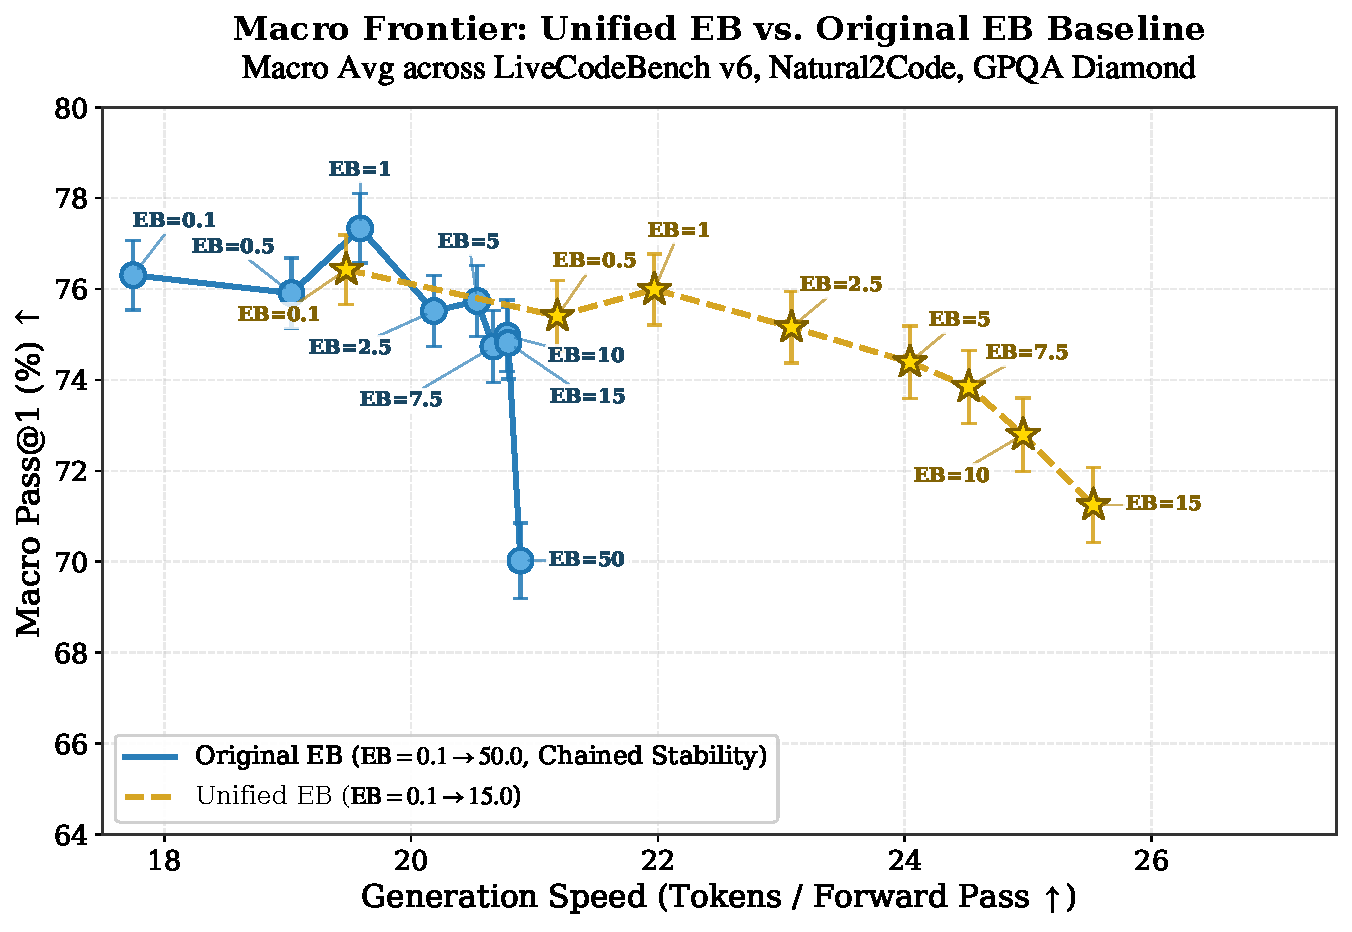
\includegraphics[height=\frontierheight]{images/fig_macro_frontier_original_vs_unified.pdf}
        \caption{Original vs.\ unified stopping.}
        \label{fig:unified-vs-orig}
    \end{subfigure}
    \hfill
    \begin{subfigure}[b]{0.51\textwidth}
        \centering
        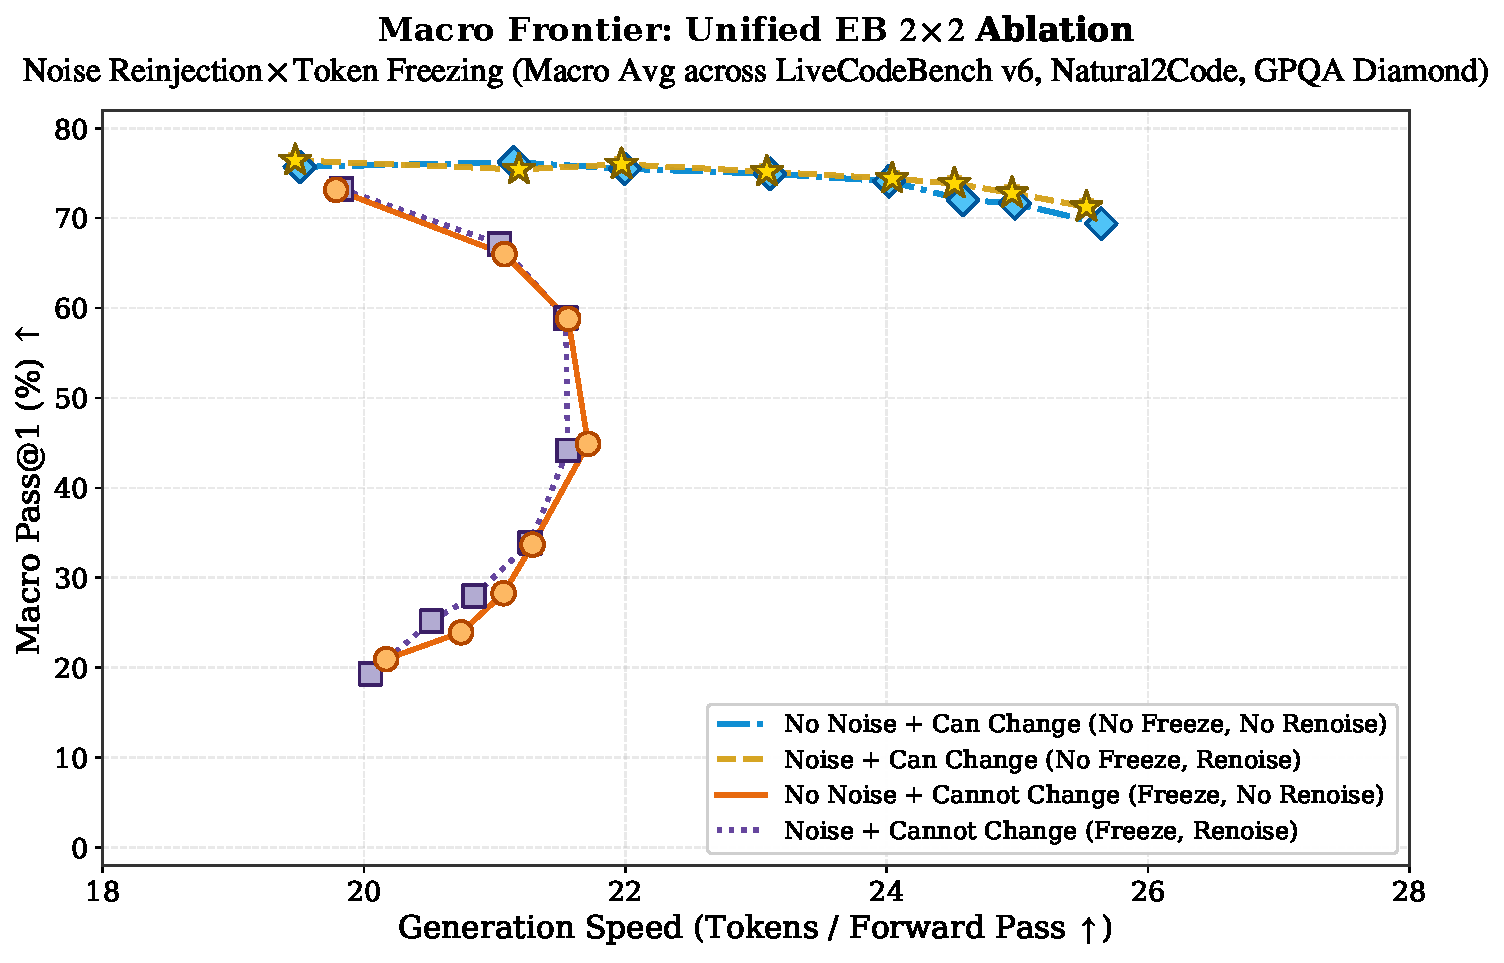
\includegraphics[height=\frontierheight]{images/fig_macro_frontier_unified_ablation_2x2.pdf}
        \caption{Frozen vs.\ base EB sampler.}
        \label{fig:frozen-eb-frontier}
    \end{subfigure}
    \caption{\textbf{(a)} The unified stopping criterion matches the original at a slight speedup. \textbf{(b)} Pareto frontier of the modified EB sampler: larger entropy bounds trade performance for throughput, and the frozen variant degrades much faster than the base version, showing that the flexibility of the uniform diffusion process drives the frontier.}
    \label{fig:eb-frontiers}
\end{figure}



\section{Committing Too Early: Frozen Tokens Cannot Self-Correct}
\label{sec:too-early}
Masked diffusion samplers treat acceptance as commitment: once a position is accepted, its token is final.
This section measures what that costs a uniform diffusion model.
One theoretical advantage of diffusion language models over autoregressive is the ability to self correct via iterative refinement.
However, the widely used masked diffusion does not allow for self correction without an explicit renoising schedule or corrector head.
Here we show that (1): DiffusionGemma exhibits self correcting properties that are driven by the model itself, not the sampler; and (2): the self correcting behavior enables it to have a robust Pareto frontier. 
\paragraph{Setup}
We focus on the EB sampler, as it is the default sampler used in \citet{team2026diffusiongemma}.
Our goal is to determine if DiffusionGemma exhibits self-correcting behavior, and whether this is driven by the model or the sampler.
To do this, we measure the macro-average of LCB v6, Natural2Code, and GPQA Diamond.
We introduce two intervention axes to investigate these questions: whether accepted tokens are "frozen" as in masked diffusion, and whether rejected tokens are renoised per the original sampler.

\paragraph{Frozen EB Sampler}
To do this, we first introduce a ``freezing'' variant of the EB sampler, where positions that are accepted under the EB rule cannot be changed later on, similar to masked diffusion.
We refer to the unmodified Unified EB sampler as ``unconstrained'', as any position can be changed regardless of whether it was already accepted under the EB rule.

\paragraph{No Noise}
To determine whether the self-correction is driven by the sampler, we additionally introduce a version of the sampler that does not renoise the rejected positions as done in the original sampler. 
If there is no additional noise injection, then the model must be able to directly correct mistakes as opposed to relying on the noise to reset incorrect positions.
This can be thought of as an Euler sampler, as it is strictly interpolating between a uniform random sample and the final sample.

\paragraph{Ablation}
Both the no noise and frozen EB sampler are orthogonal directions of intervention. Thus we ablate over all four combinations and show the results in Figure \ref{fig:frozen-eb-frontier}.
For each possible combination, we do a sweep over various entropy bound values to examine how they are affected by more relaxed thresholds. 
For the unconstrained variants, we also track the empirical frequencies of each position being altered during the denoising trajectory after the initial acceptance under the EB rule.
We show these position volatility metrics in Figure~\ref{fig:wasted} (bottom row).

% \begin{figure}[t]
%     \centering
%     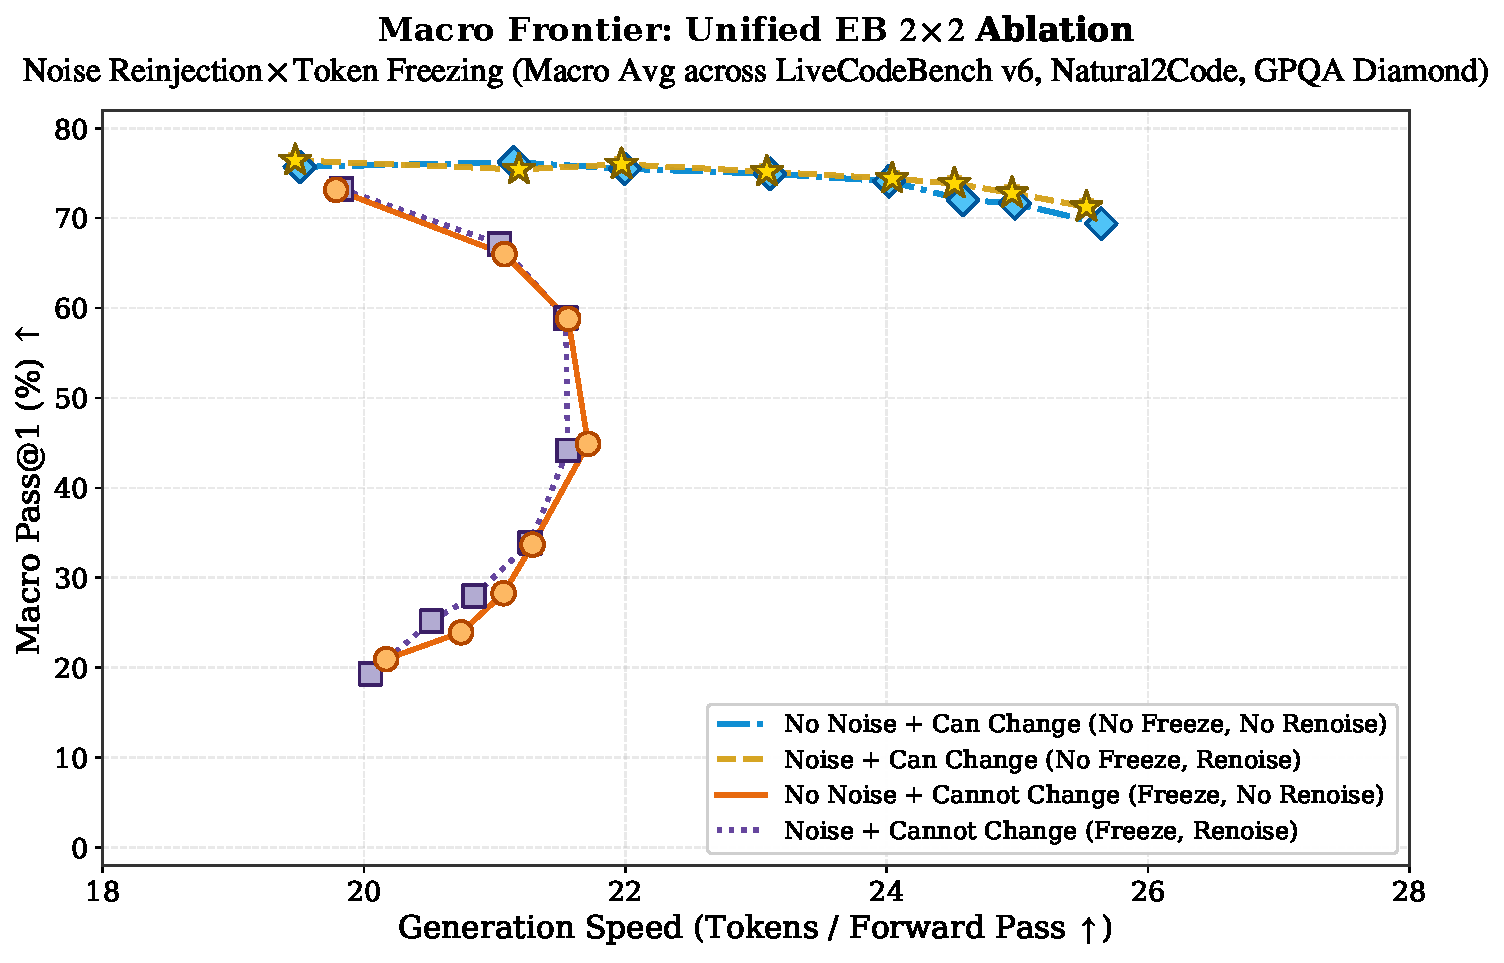
\includegraphics[width=1.0\linewidth]{images/fig_macro_frontier_unified_ablation_2x2.pdf}
%     \caption{We show the frontier for the modified DiffusionGemma EB sampler, where the entropy bound controls both the early stopping criterion and the commitment within a block. We observe that as the entropy bound grows, the sampler is able to increase throughput by sacrificing performance, producing a pareto frontier. The frozen variant of the EB sampler deteriorates performance much more rapidly than the base version, demonstrating that the flexibility of the uniform diffusion process contributes to the strong pareto frontier of DiffusionGemma.}
%     \label{fig:frozen-eb-frontier}
% \end{figure}


\paragraph{Results}
We observe that for each adaptive variant, the unconstrained sampler achieves a superior pareto frontier than the frozen sampler, and this gap increases with further relaxation of the thresholds.
At the loosest bound, the frozen variants fall to about 20\% macro Pass@1, while the unconstrained variants stay near 70\%.
Furthermore, the number of positions that change after initial acceptance increases with higher entropy thresholds, and is relatively unaffected by whether the sampler uses noise injection.
At the default bound of $0.1$, roughly 97\% to 99\% of accepted positions never change, so the default sampler behaves much like a frozen one; revisions become frequent only as the bound is relaxed.
This indicates that 1) the model does rely on self correction, as removing this deteriorates performance at relaxed thresholds; and 2) the self-correction is driven by the changes in the model's posterior as opposed to renoising, as removing noise does not alter post-acceptance behavior.

The design rule that follows is that acceptance must not be final: an accepted token should stay free to change until it is committed to the KV cache.


\section{Committing Too Late: Converged Tokens Waste Denoising Slots}
\label{sec:too-late}
Block samplers sit at the other extreme: no token is committed until the whole block has converged.
Here we examine the order in which DiffusionGemma accepts tokens under the Unified EB sampler.
We observe that DiffusionGemma exhibits a sampling order strongly biased towards autoregressive generation.
This autoregressive bias results in many denoising slots within a canvas being "wasted" on tokens that have already converged.
As a result, a form of rolling sampler where the window moves incrementally through the sequence rather than block by block becomes increasingly appealing as a way to extend the pareto frontier.

% ---------------------------------------------------------------
% Block vs rolling sampler: where the denoising slots go.
%
% Palette is shared with the concept figure (v12):
%   white  = already encoded, in the KV cache   (was gray here)
%   gray   = not yet admitted                   (was white here)
%   teal   = denoising slot
%   amber  = accepted on this pass              (was blue here)
%   brick  = wasted: re-denoised while waiting for its prefix
% The white/gray swap matters: in the concept figure white always means
% "settled, never recomputed" and gray always means "not admitted yet".
%
% Requires: \usepackage{tikz}
% ---------------------------------------------------------------
\begin{figure}[tbp]
\centering
\begin{tikzpicture}[x=0.205cm, y=0.205cm]

\definecolor{cwinfill}{HTML}{9FE1CB}
\definecolor{cwinedge}{HTML}{0F6E56}
\definecolor{camber}{HTML}{E8A13C}
\definecolor{camberedge}{HTML}{A96A0B}
\definecolor{cwaste}{HTML}{C0553C}
\definecolor{cwasteedge}{HTML}{7A2E1C}
\definecolor{cnoise}{HTML}{D3D1C7}
\definecolor{cnoiseedge}{HTML}{888780}
\definecolor{cclean}{HTML}{FFFFFF}
\definecolor{ccleanedge}{HTML}{B4B4A9}
\definecolor{cframe}{HTML}{2B5E94}

% Exact tints from the concept figure: the strip's cells are cwinfill!(30..100)
% with cwinedge, camber!45 with camberedge, cnoise with cnoiseedge, cclean with
% ccleanedge; the mask's window block is cwinfill!65.  A uniform denoising slot
% here therefore takes cwinfill!65.
% 1 = denoising, 2 = accepted this pass, 3 = accepted but re-denoised,
% 4 = in KV cache, 5 = not admitted
\newcommand{\gridcell}[3]{%
  \ifcase#3\relax
  \or \fill[cwinfill!65, draw=cwinedge,   line width=0.3pt, rounded corners=0.5pt] (#1, -#2) rectangle ++(0.88, -0.88);
  \or \fill[camber!45,   draw=camberedge, line width=0.3pt, rounded corners=0.5pt] (#1, -#2) rectangle ++(0.88, -0.88);
  \or \fill[cwaste,      draw=cwasteedge, line width=0.3pt, rounded corners=0.5pt] (#1, -#2) rectangle ++(0.88, -0.88);
  \or \fill[cclean,      draw=ccleanedge, line width=0.3pt, rounded corners=0.5pt] (#1, -#2) rectangle ++(0.88, -0.88);
  \or \fill[cnoise,      draw=cnoiseedge, line width=0.3pt, rounded corners=0.5pt] (#1, -#2) rectangle ++(0.88, -0.88);
  \fi}

% \gridrow{x shift}{row}{window lo}{window hi}
%   cols [0, lo)  : already encoded, in the KV cache (white)
%   cols [lo, hi) : denoised on this pass            (teal)
%   cols [hi, 24) : not yet admitted                 (gray)
\newcommand{\gridrow}[4]{%
  \foreach \c in {0,...,23} {%
    \pgfmathtruncatemacro{\sty}{\c<#3 ? 4 : (\c<#4 ? 1 : 5)}%
    \pgfmathsetmacro{\xpos}{\c + #1}%
    \gridcell{\xpos}{#2}{\sty}%
  }}

% \gridmarks{x shift}{row}{style}{column list} -- repaint individual cells of a row.
% Acceptance is out of order, so these sets are not contiguous ranges.
% (Do not call this \marks: that is an e-TeX primitive.)
\newcommand{\gridmarks}[4]{%
  \foreach \c in {#4} {%
    \pgfmathsetmacro{\xpos}{\c + #1}%
    \gridcell{\xpos}{#2}{#3}%
  }}

% ---------- inline legend swatches (same vocabulary as the concept figure) ----------
\newcommand{\keydenoise}{\begin{tikzpicture}[baseline=-0.5ex, x=0.30cm, y=0.30cm]
  \fill[cwinfill!65, draw=cwinedge, line width=0.3pt, rounded corners=0.5pt] (0,-0.5) rectangle ++(0.88,1);
\end{tikzpicture}}
\newcommand{\keyaccept}{\begin{tikzpicture}[baseline=-0.5ex, x=0.30cm, y=0.30cm]
  \fill[camber!45, draw=camberedge, line width=0.3pt, rounded corners=0.5pt] (0,-0.5) rectangle ++(0.88,1);
\end{tikzpicture}}
\newcommand{\keywaste}{\begin{tikzpicture}[baseline=-0.5ex, x=0.30cm, y=0.30cm]
  \fill[cwaste, draw=cwasteedge, line width=0.3pt, rounded corners=0.5pt] (0,-0.5) rectangle ++(0.88,1);
\end{tikzpicture}}
\newcommand{\keycache}{\begin{tikzpicture}[baseline=-0.5ex, x=0.30cm, y=0.30cm]
  \fill[cclean, draw=ccleanedge, line width=0.3pt, rounded corners=0.5pt] (0,-0.5) rectangle ++(0.88,1);
\end{tikzpicture}}
\newcommand{\keyunadmitted}{\begin{tikzpicture}[baseline=-0.5ex, x=0.30cm, y=0.30cm]
  \fill[cnoise, draw=cnoiseedge, line width=0.3pt, rounded corners=0.5pt] (0,-0.5) rectangle ++(0.88,1);
\end{tikzpicture}}

% ===== Panel (a), left: block sampler, three blocks of b = 8, 19 passes =====
\node[anchor=west, font=\footnotesize\bfseries] at (0, 1.5) {(a) Block sampler, $b=8$: 19 passes};

% Block 1 (cols 0-7): accepts {0,3}, {1,2}, {4,6}, {5,7}
\gridrow{0}{0}{0}{8}
\gridrow{0}{1}{0}{8}
\gridrow{0}{2}{0}{8}                     \gridmarks{0}{2}{2}{0,3}
\gridrow{0}{3}{0}{8} \gridmarks{0}{3}{3}{0,3}          \gridmarks{0}{3}{2}{1,2}
\gridrow{0}{4}{0}{8} \gridmarks{0}{4}{3}{0,1,2,3}      \gridmarks{0}{4}{2}{4,6}
\gridrow{0}{5}{0}{8} \gridmarks{0}{5}{3}{0,1,2,3,4,6}  \gridmarks{0}{5}{2}{5,7}
% Block 2 (cols 8-15): a slower block, accepts {8,11}, {9}, {10,13}, {12,14}, {15}
\gridrow{0}{6}{8}{16}
\gridrow{0}{7}{8}{16}
\gridrow{0}{8}{8}{16}                        \gridmarks{0}{8}{2}{8,11}
\gridrow{0}{9}{8}{16}  \gridmarks{0}{9}{3}{8,11}             \gridmarks{0}{9}{2}{9}
\gridrow{0}{10}{8}{16} \gridmarks{0}{10}{3}{8,9,11}          \gridmarks{0}{10}{2}{10,13}
\gridrow{0}{11}{8}{16} \gridmarks{0}{11}{3}{8,9,10,11,13}    \gridmarks{0}{11}{2}{12,14}
\gridrow{0}{12}{8}{16} \gridmarks{0}{12}{3}{8,9,10,11,12,13,14} \gridmarks{0}{12}{2}{15}
% Block 3 (cols 16-23): accepts {16,19}, {17,18}, {20,22}, {21,23}
\gridrow{0}{13}{16}{24}
\gridrow{0}{14}{16}{24}
\gridrow{0}{15}{16}{24}                          \gridmarks{0}{15}{2}{16,19}
\gridrow{0}{16}{16}{24} \gridmarks{0}{16}{3}{16,19}              \gridmarks{0}{16}{2}{17,18}
\gridrow{0}{17}{16}{24} \gridmarks{0}{17}{3}{16,17,18,19}        \gridmarks{0}{17}{2}{20,22}
\gridrow{0}{18}{16}{24} \gridmarks{0}{18}{3}{16,17,18,19,20,22}  \gridmarks{0}{18}{2}{21,23}

% Block boundaries
\foreach \x in {7.94, 15.94} {
  \draw[cframe, dashed, line width=0.4pt] (\x, 0.3) -- (\x, -19.2);
}
\node[anchor=east, font=\scriptsize] at (-0.5, -0.44) {$t=1$};
\node[anchor=east, font=\scriptsize] at (-0.5, -18.44) {$t=19$};

% ===== Panel (b), right: rolling sampler, w = 8, 13 passes =====
\node[anchor=west, font=\footnotesize\bfseries] at (29.5, 1.5) {(b) Rolling sampler, $w=8$: 13 passes};

\gridrow{29.5}{0}{0}{8}
\gridrow{29.5}{1}{0}{8}
\gridrow{29.5}{2}{0}{8}                          \gridmarks{29.5}{2}{2}{0,3}
\gridrow{29.5}{3}{1}{9}   \gridmarks{29.5}{3}{3}{3}          \gridmarks{29.5}{3}{2}{1,2}
\gridrow{29.5}{4}{4}{12}                         \gridmarks{29.5}{4}{2}{4,6}
\gridrow{29.5}{5}{5}{13}  \gridmarks{29.5}{5}{3}{6}          \gridmarks{29.5}{5}{2}{5,7,8}
\gridrow{29.5}{6}{9}{17}                         \gridmarks{29.5}{6}{2}{9,12}
\gridrow{29.5}{7}{10}{18} \gridmarks{29.5}{7}{3}{12}         \gridmarks{29.5}{7}{2}{10,11}
\gridrow{29.5}{8}{13}{21}                        \gridmarks{29.5}{8}{2}{13,14,17}
% t=10: 16 and 18 are accepted but 15 is not, so the prefix -- and the window -- cannot move
\gridrow{29.5}{9}{15}{23} \gridmarks{29.5}{9}{3}{17}         \gridmarks{29.5}{9}{2}{16,18}
% t=11: 15 resolves and five positions flush to the cache at once
\gridrow{29.5}{10}{15}{23} \gridmarks{29.5}{10}{3}{16,17,18} \gridmarks{29.5}{10}{2}{15,19}
\gridrow{29.5}{11}{20}{24}                       \gridmarks{29.5}{11}{2}{20,22}
\gridrow{29.5}{12}{21}{24} \gridmarks{29.5}{12}{3}{22}       \gridmarks{29.5}{12}{2}{21,23}

\node[anchor=east, font=\scriptsize] at (29.0, -0.44) {$t=1$};
\node[anchor=east, font=\scriptsize] at (29.0, -12.44) {$t=13$};

% ===== Legend: measured by LaTeX and centred on the two grids (x = 0..53.4) =====
\node[anchor=north, font=\scriptsize, inner sep=0pt] at (26.7, -20.4) {%
  \begin{tabular}{@{}l@{~}l@{\hspace{1.8em}}l@{~}l@{\hspace{1.8em}}l@{~}l@{}}
    \keydenoise & denoising slot   & \keyaccept     & accepted on this pass &
    \keywaste   & wasted: re-denoised while waiting \\[2.5pt]
    \keycache   & in the KV cache  & \keyunadmitted & not yet admitted      &
                &                                    \\
  \end{tabular}};

\end{tikzpicture}
\caption{\textbf{Where the denoising slots go.} Both samplers denoise a
width-$8$ window per pass in the same order, and the colours are those of
Figure~\ref{fig:algorithm-concept}: teal = still denoising, amber = accepted
on this pass, white = already encoded and in the KV cache, gray = not yet
admitted.  Brick marks a slot spent re-denoising a position that was already
accepted but is still waiting for its prefix, that is, wasted work.
\textbf{(a)} The block sampler appends only once the block is fully resolved,
so converged positions idle and each block re-pays warm-up.  \textbf{(b)} The
rolling sampler appends the accepted prefix immediately and admits fresh
positions in its place, wasting far fewer slots.}
\label{fig:block-vs-rolling}
\end{figure}

\paragraph{Defining Redundant Computations}
Here we define what constitutes a redundant computation.
Our goal is to measure the computations that could conceivably be omitted without drastically impacting the model's behavior.
Thus we define wasted denoising slots as positions that have already converged and are part of a contiguous prefix that could be appended to the KV cache.
We illustrate this definition in Figure \ref{fig:block-vs-rolling}, against the ideal sampler that commits them to the KV cache and avoids redundant denoising steps.

\begin{figure}[tbp]
    \centering
    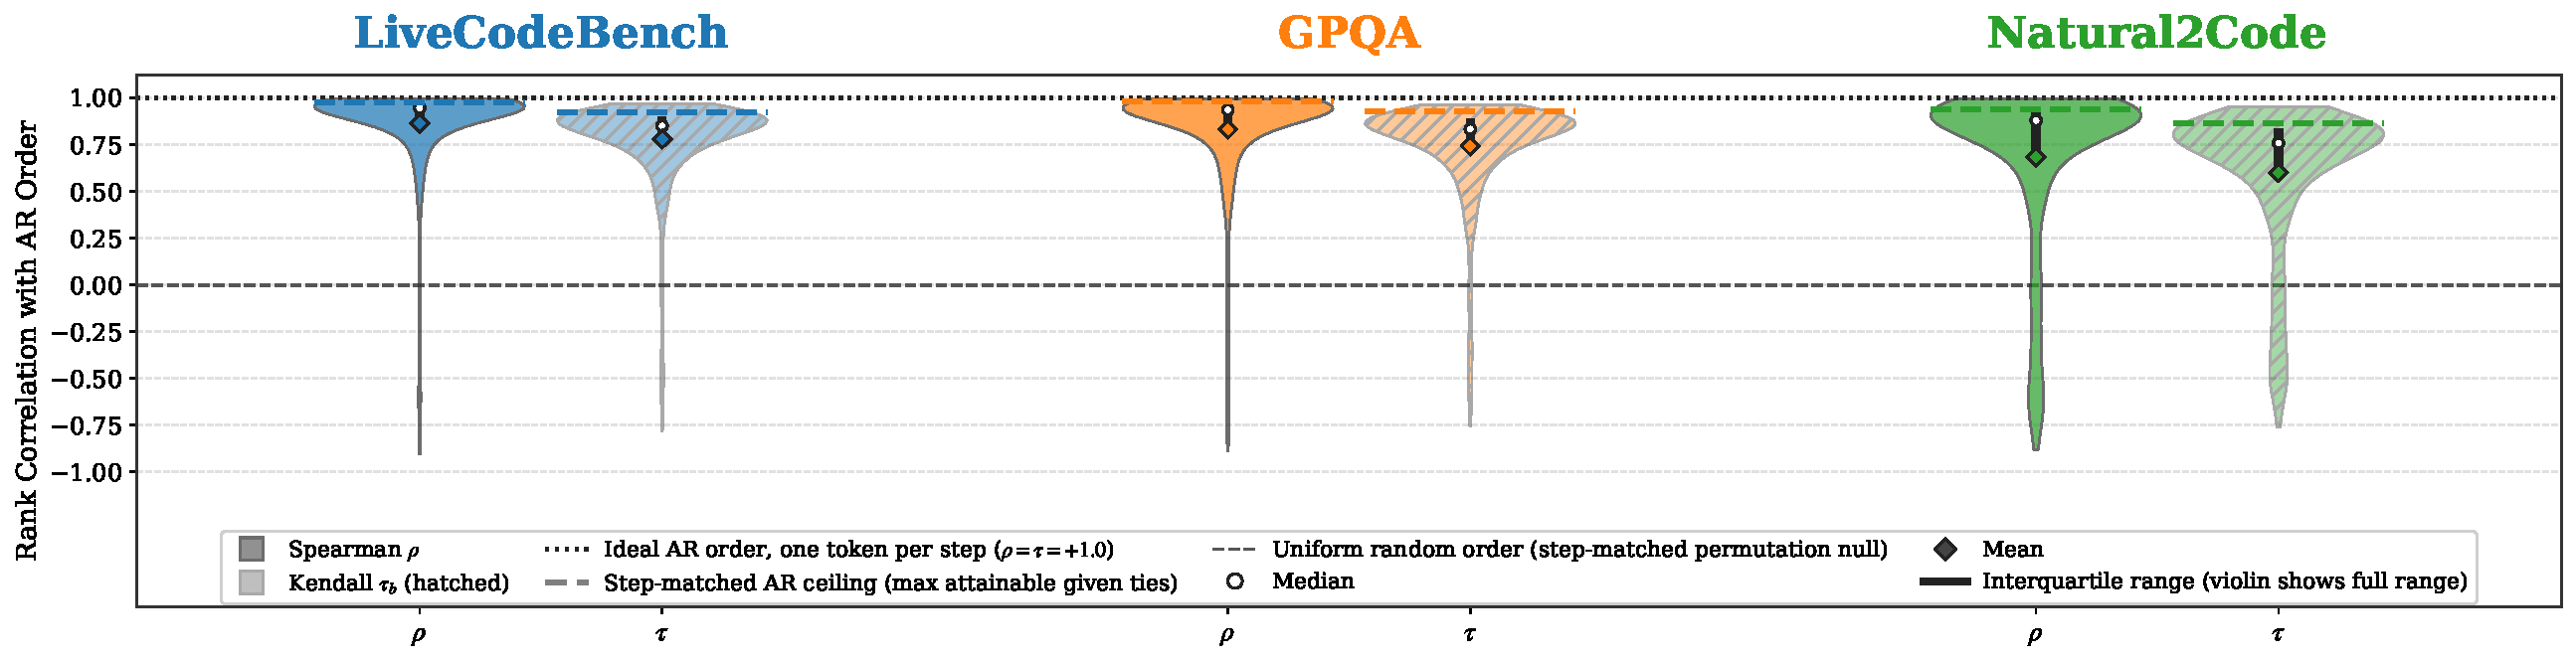
\includegraphics[width=\linewidth]{images/fig_ar_order_correlation_eb0.1_renoise.pdf}

    \vspace{8pt}

    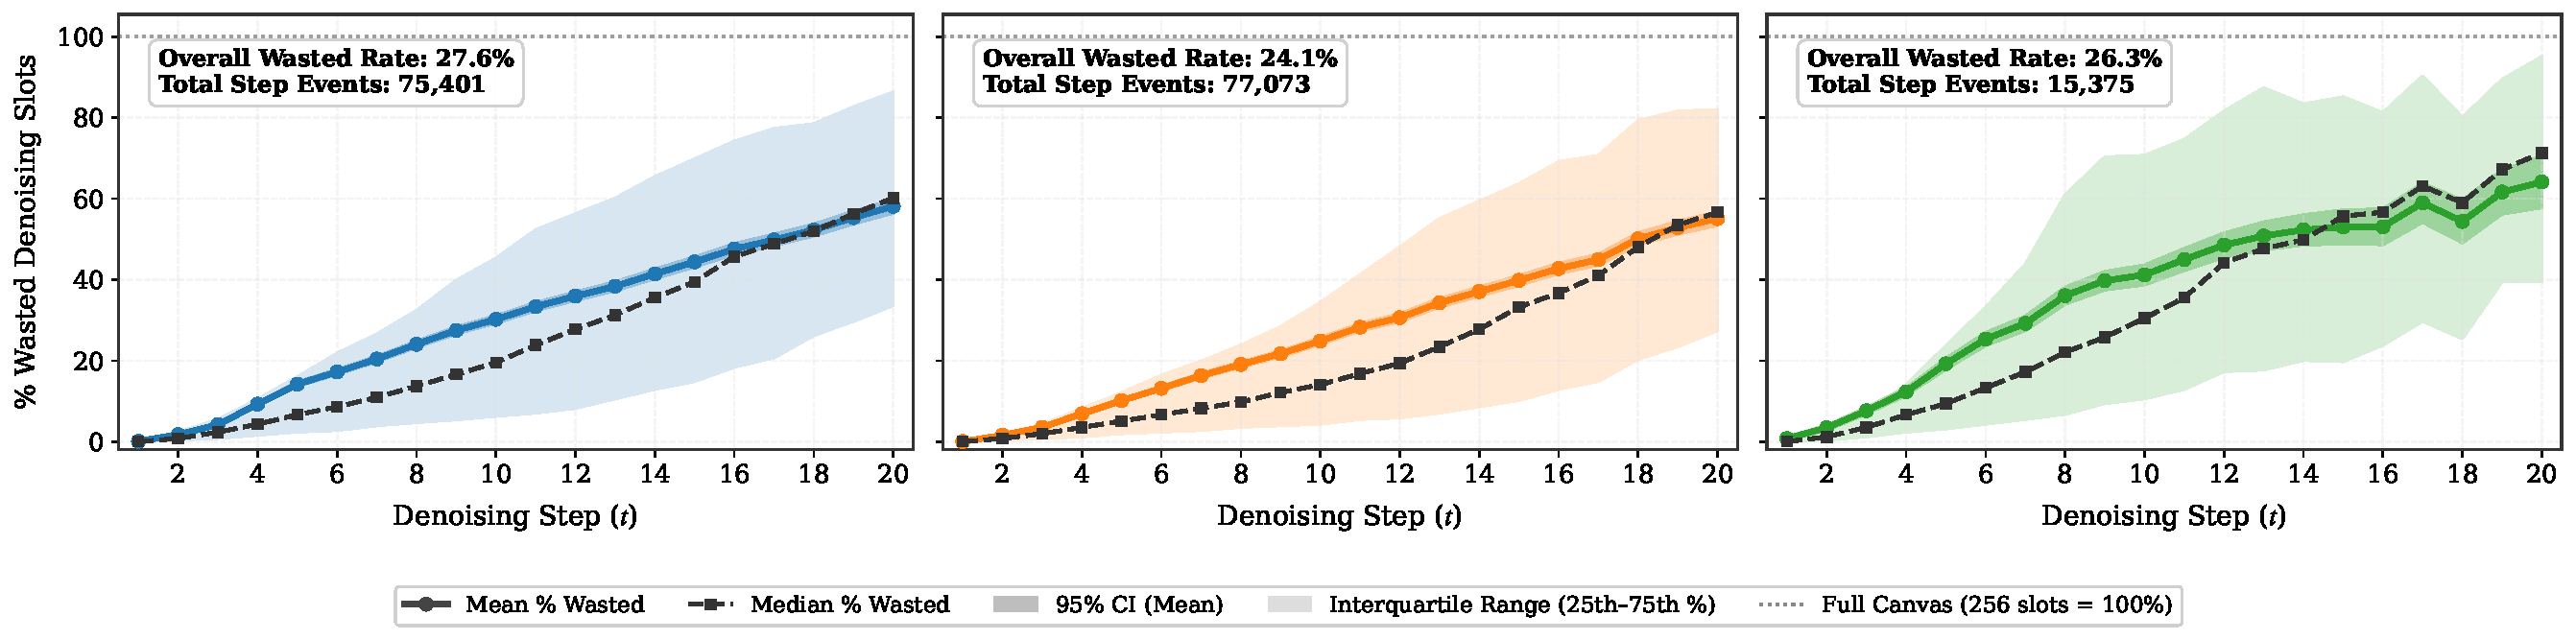
\includegraphics[width=\linewidth]{images/wasted_canvas_slots_lcb_gpqa_n2c.pdf}

    \vspace{8pt}

    % trim crops the task titles baked into the image; the top row already names the tasks
    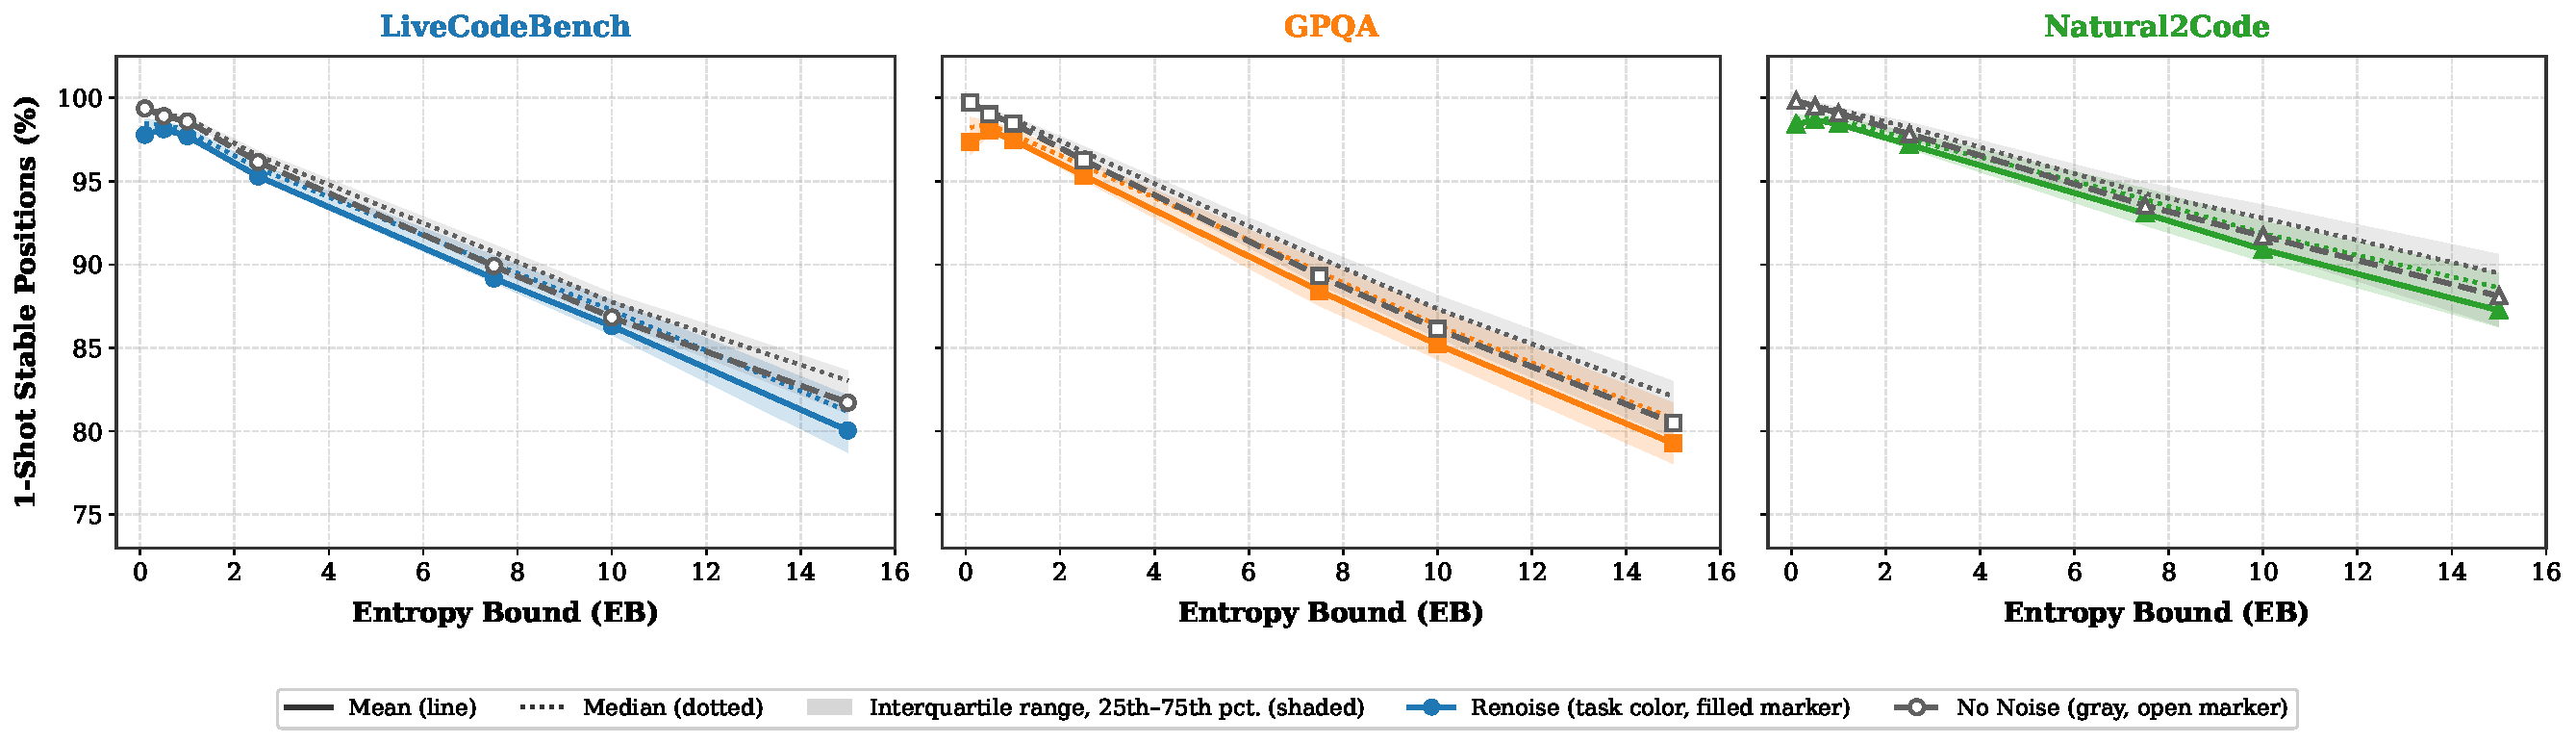
\includegraphics[width=\linewidth,trim=0 0 0 23.5pt,clip]{images/fig_1shot_stability_1x2_row.pdf}
    \caption{Columns show LiveCodeBench, GPQA Diamond, and Natural2Code in every row. \textbf{Top row:} Spearman $\rho$ and Kendall $\tau$ between the acceptance order of the DiffusionGemma EB sampler and the AR generation order; across all tasks the sampler is strongly biased towards left-to-right order. \textbf{Middle row:} Number of wasted denoising slots averaged across canvases for LCB v6, GPQA Diamond and Natural2Code. For a given sampling step, a slot is wasted if it belongs to a contiguous prefix that has already converged to its final token. Past 10 denoising steps, over half of the canvas slots are wasted. \textbf{Bottom row:} Accepted tokens are revised more often at higher entropy bounds (in both argmax and sampled-token stability), independent of renoising.}
    \label{fig:wasted}
\end{figure}


\paragraph{Experimental Setup}
We run the Unified EB sampler on LCB v6, GPQA Diamond and Natural2Code. We track the trajectories of each denoising block, and consider a position as converged when it realizes the value that ends up being committed to the KV cache.

\paragraph{Results}
In Figure~\ref{fig:wasted} (top row), we observe that the convergence ordering of positions is very correlated with left-to-right order. This explains the behavior of wasted denoising slots in Figure~\ref{fig:wasted} (middle row), where we observe that the percentage of wasted slots increases monotonically during the denoising trajectory.  

\citet{asaria2026neither} previously observed this autoregressive bias in the DiffusionGemma sampler. 
This is not a model specific quirk: this aligns with many general observations of the sampling behavior for confidence-based samplers for large scale diffusion language models. 
\citet{kim2026interface} demonstrates that confidence based samplers tend to generate samples that are very similar to those produced by left-to-right autoregressive order. 
Other works demonstrate that the ordering itself is highly left to right and provide various explanations for why \citep{gong2026diffucoder, lu2026adablock, yao2026decoding}.

The design rule here mirrors the previous one: a token that has reached its final value should not wait for the rest of the block.
The two rules pull in opposite directions, since committing later leaves more room for revision while committing earlier wastes fewer slots.
Section~\ref{sec:method} introduces a sampler that sits between the two extremes.


\section{RES: A Rolling Sampler}
\label{sec:method}
Here we introduce the Rolling Entropy Sampler (RES), a sampler that commits tokens neither at acceptance nor at the end of the block.
The core mechanism is simple: instead of waiting for the entire block to converge, RES encodes any sufficiently long contiguous prefix of accepted tokens, appends it to the KV cache, and refills the freed slots with fresh noise.
Positions outside the committed prefix, accepted or not, remain free to change.
Figure~\ref{fig:algorithm-concept} illustrates the method.
% ---------------------------------------------------------------
% Concept figure v12: rolling sampler + per-step attention mask.
%
% One row per decoding step.  Each row carries
%   left  : the sequence, with positions pinned to columns
%   right : the attention mask in force on that pass
% and the mask panel covers exactly the ten positions inside the dashed
% frame on its left, so the two halves are the same object twice.
%
% Fixed compute budget: every pass processes TEN positions,
%   encoded prefix (p slots, committed last pass, encoded causally)
%   + denoising window (10 - p slots).
% Hence p = 0, 2, 4 gives denoising widths 10, 8, 6 and masks that are
% all 10 x 10: fully bidirectional, then 2 causal, then 4 causal.
% The block slides forward by however many slots graduated into the KV
% cache on the previous pass, so the stride is data dependent.
%
% Colour vocabulary is shared by the two halves:
%   white  = already encoded, sitting in the KV cache (never recomputed)
%   amber  = committed, being encoded on this pass
%   teal   = denoising slot (saturation = noise level)
%   gray   = not yet admitted, holds an arbitrary noise token
%   pale   = masked out (mask panels only)
% Indicators:
%   amber border = accepted on this pass
%   amber dot    = accepted on an earlier pass, awaiting the contiguous prefix
%
% Requires: \usepackage{tikz}   (no extra libraries)
% ---------------------------------------------------------------
\begin{figure}[tbp]
\centering
\begin{tikzpicture}[x=0.36cm, y=0.36cm]

\definecolor{cclean}{HTML}{FFFFFF}
\definecolor{ccleanedge}{HTML}{B4B4A9}
\definecolor{cwinedge}{HTML}{0F6E56}
\definecolor{cwinfill}{HTML}{9FE1CB}
\definecolor{cnoise}{HTML}{D3D1C7}
\definecolor{cnoiseedge}{HTML}{888780}
\definecolor{cframe}{HTML}{2B5E94}
\definecolor{camber}{HTML}{E8A13C}
\definecolor{camberedge}{HTML}{A96A0B}
\definecolor{mempty}{HTML}{F5F4EF}
\definecolor{memptyedge}{HTML}{C9C7BE}

% ---------- sequence cells (outer coordinate system) ----------
% #1 = column, #2 = row baseline, last arg = character ({} for a space)
\newcommand{\cellclean}[3]{%
  \fill[cclean, draw=ccleanedge, line width=0.4pt, rounded corners=1pt] (#1, #2) rectangle ++(0.9, 1);
  \node[font=\scriptsize\ttfamily, inner sep=0pt, text=black] at (#1+0.45, #2+0.5) {#3};}
\newcommand{\cellwin}[4]{%
  \fill[cwinfill!#3, draw=cwinedge, line width=0.4pt, rounded corners=1pt] (#1, #2) rectangle ++(0.9, 1);
  \node[font=\scriptsize\ttfamily, inner sep=0pt, text=black] at (#1+0.45, #2+0.5) {#4};}
\newcommand{\cellnoise}[3]{%
  \fill[cnoise, draw=cnoiseedge, line width=0.4pt, rounded corners=1pt] (#1, #2) rectangle ++(0.9, 1);
  \node[font=\scriptsize\ttfamily, inner sep=0pt, text=cnoiseedge] at (#1+0.45, #2+0.5) {#3};}
\newcommand{\cellamber}[3]{%
  \fill[camber!45, draw=camberedge, line width=0.6pt, rounded corners=1pt] (#1, #2) rectangle ++(0.9, 1);
  \node[font=\scriptsize\ttfamily, inner sep=0pt, text=black] at (#1+0.45, #2+0.5) {#3};}
\newcommand{\acceptmark}[2]{\draw[camberedge, line width=1.1pt, rounded corners=1pt] (#1+0.03, #2+0.03) rectangle ++(0.84, 0.94);}
\newcommand{\acceptdot}[2]{\fill[camberedge] (#1+0.45, #2+0.17) circle (0.12);}
% dashed frame around the ten processed cells starting at column #1, row #2
\newcommand{\passframe}[2]{%
  \draw[cframe, line width=1.1pt, rounded corners=2pt, dash pattern=on 4pt off 2pt]
    (#1-0.15, #2-0.25) rectangle (#1+10.05, #2+1.25);}
% measuring bracket under the strip: columns #1..#2 of the row based at #3
\newcommand{\seqbracket}[4]{%
  \draw[line width=0.3pt] (#1, #3-0.55) -- (#1, #3-0.90) -- (#2+0.9, #3-0.90) -- (#2+0.9, #3-0.55);
  \node[font=\tiny, anchor=north, inner sep=1.5pt] at ({(#1+#2+0.9)/2}, #3-0.90) {#4};}

% ---------- attention-mask panel ----------
% #1 = first position drawn, #2 = last position drawn,
% #3 = last position of the encoded prefix; pass #1-1 for "no prefix",
% #4 = x of the panel's top-left corner in cm, #5 = y of it in cm.
% Rows are queries, columns are keys.  Prefix rows see only prefix keys at
% or before them (causal); denoising rows see every position in the block.
\newcommand{\maskpanel}[5]{%
\begin{scope}[shift={(#4cm,#5cm)}, x=0.19cm, y=0.19cm]
  \foreach \q in {#1,...,#2}{%
    \foreach \k in {#1,...,#2}{%
      \pgfmathtruncatemacro{\ii}{\k-#1}%
      \pgfmathtruncatemacro{\jj}{\q-#1}%
      \ifnum\q>#3\relax
        \ifnum\k>#3\relax
          \fill[cwinfill!65, draw=cwinedge, line width=0.25pt, rounded corners=0.4pt] (\ii,-\jj) rectangle ++(0.88,-0.88);
        \else
          \fill[camber!20, draw=camberedge, line width=0.25pt, rounded corners=0.4pt] (\ii,-\jj) rectangle ++(0.88,-0.88);
        \fi
      \else
        \ifnum\k>\q\relax
          \fill[mempty, draw=memptyedge, line width=0.25pt, rounded corners=0.4pt] (\ii,-\jj) rectangle ++(0.88,-0.88);
        \else
          \fill[camber!55, draw=camberedge, line width=0.25pt, rounded corners=0.4pt] (\ii,-\jj) rectangle ++(0.88,-0.88);
        \fi
      \fi}}%
  \pgfmathtruncatemacro{\cc}{#3-#1+1}%
  \pgfmathtruncatemacro{\nn}{#2-#1+1}%
  \ifnum\cc>0\relax
    \draw[dashed, line width=0.4pt] (\cc-0.06, 0.5) -- (\cc-0.06, -\nn-0.1);
    \draw[dashed, line width=0.4pt] (-0.5, -\cc+0.06) -- (\nn+0.1, -\cc+0.06);
    \draw[camberedge, line width=0.8pt, rounded corners=0.6pt] (-0.06, 0.06) rectangle (\cc-0.12, -\cc+0.12);
  \fi
\end{scope}}
% measuring brackets under a mask panel (drawn once, for the bottom panel)
% #1 = prefix width in cells, #2 = panel width in cells, #3/#4 = corner in cm
\newcommand{\maskbrackets}[4]{%
\begin{scope}[shift={(#3cm,#4cm)}, x=0.19cm, y=0.19cm]
  \ifnum#1>0\relax
    \draw[line width=0.3pt] (0,-#2-0.5) -- (0,-#2-0.9) -- (#1-0.12,-#2-0.9) -- (#1-0.12,-#2-0.5);
    \node[font=\tiny, anchor=north, inner sep=1.5pt] at (#1/2-0.06, -#2-0.9) {prefix};
  \fi
  \draw[line width=0.3pt] (#1,-#2-0.5) -- (#1,-#2-0.9) -- (#2-0.12,-#2-0.9) -- (#2-0.12,-#2-0.5);
  \node[font=\tiny, anchor=north, inner sep=1.5pt] at ({(#1+#2)/2-0.06}, -#2-0.9) {window};
\end{scope}}

% ---------- inline legend swatches ----------
\newcommand{\keyencoded}{\begin{tikzpicture}[baseline=-0.5ex, x=0.36cm, y=0.36cm]
  \fill[cclean, draw=ccleanedge, line width=0.4pt, rounded corners=1pt] (0,-0.5) rectangle ++(0.9,1);
\end{tikzpicture}}
\newcommand{\keyaccepted}{\begin{tikzpicture}[baseline=-0.5ex, x=0.36cm, y=0.36cm]
  \fill[cwinfill!30, draw=cwinedge, line width=0.4pt, rounded corners=1pt] (0,-0.5) rectangle ++(0.9,1);
  \draw[camberedge, line width=1.1pt, rounded corners=1pt] (0.03,-0.47) rectangle ++(0.84,0.94);
\end{tikzpicture}}
\newcommand{\keywaiting}{\begin{tikzpicture}[baseline=-0.5ex, x=0.36cm, y=0.36cm]
  \fill[cwinfill!30, draw=cwinedge, line width=0.4pt, rounded corners=1pt] (0,-0.5) rectangle ++(0.9,1);
  \fill[camberedge] (0.45,-0.33) circle (0.12);
\end{tikzpicture}}
\newcommand{\keyprefix}{\begin{tikzpicture}[baseline=-0.5ex, x=0.36cm, y=0.36cm]
  \fill[camber!45, draw=camberedge, line width=0.6pt, rounded corners=1pt] (0,-0.5) rectangle ++(0.9,1);
\end{tikzpicture}}
\newcommand{\keynoise}{\begin{tikzpicture}[baseline=-0.5ex, x=0.36cm, y=0.36cm]
  \fill[cnoise, draw=cnoiseedge, line width=0.4pt, rounded corners=1pt] (0,-0.5) rectangle ++(0.9,1);
  \node[font=\scriptsize\ttfamily, inner sep=0pt, text=cnoiseedge] at (0.45,0) {k};
\end{tikzpicture}}
\newcommand{\keymcausal}{\begin{tikzpicture}[baseline=-0.5ex, x=0.36cm, y=0.36cm]
  \fill[camber!55, draw=camberedge, line width=0.4pt, rounded corners=1pt] (0,-0.5) rectangle ++(0.9,1);
\end{tikzpicture}}
\newcommand{\keymcross}{\begin{tikzpicture}[baseline=-0.5ex, x=0.36cm, y=0.36cm]
  \fill[camber!20, draw=camberedge, line width=0.4pt, rounded corners=1pt] (0,-0.5) rectangle ++(0.9,1);
\end{tikzpicture}}
\newcommand{\keymbidi}{\begin{tikzpicture}[baseline=-0.5ex, x=0.36cm, y=0.36cm]
  \fill[cwinfill!65, draw=cwinedge, line width=0.4pt, rounded corners=1pt] (0,-0.5) rectangle ++(0.9,1);
\end{tikzpicture}}
\newcommand{\keymempty}{\begin{tikzpicture}[baseline=-0.5ex, x=0.36cm, y=0.36cm]
  \fill[mempty, draw=memptyedge, line width=0.4pt, rounded corners=1pt] (0,-0.5) rectangle ++(0.9,1);
\end{tikzpicture}}

% ===================== step t : block 8-17, prefix 0, denoise 10 =====================
\node[anchor=east, font=\small\bfseries] at (-0.60, 0.50) {step $t$};
\cellclean{0}{0}{t}
\cellclean{1}{0}{h}
\cellclean{2}{0}{e}
\cellclean{3}{0}{}
\cellclean{4}{0}{c}
\cellclean{5}{0}{a}
\cellclean{6}{0}{t}
\cellclean{7}{0}{}
\cellwin{8}{0}{30}{m}
\cellwin{9}{0}{30}{e}
\cellwin{10}{0}{55}{r}
\cellwin{11}{0}{30}{w}
\cellwin{12}{0}{70}{s}
\cellwin{13}{0}{90}{}
\cellwin{14}{0}{100}{q}
\cellwin{15}{0}{100}{7}
\cellwin{16}{0}{100}{x}
\cellwin{17}{0}{100}{v}
\cellnoise{18}{0}{9}
\cellnoise{19}{0}{k}
\cellnoise{20}{0}{z}
\cellnoise{21}{0}{3}
\cellnoise{22}{0}{b}
\cellnoise{23}{0}{5}
\acceptmark{8}{0}
\acceptmark{9}{0}
\acceptmark{11}{0}
\passframe{8}{0}
\seqbracket{8}{17}{0}{10 positions per pass}
\maskpanel{8}{17}{7}{9.25}{1.13}

\node[font=\scriptsize, anchor=south, text=ccleanedge!60!black] at (3.95, 1.32) {KV cache};
\node[cframe, font=\scriptsize, anchor=south] at (12.95, 1.32) {processed this pass};
\node[cnoiseedge, font=\scriptsize, anchor=south] at (20.95, 1.32) {not yet admitted};
\node[font=\scriptsize, anchor=south] at (10.20cm, 1.57cm) {attention mask};
\node[font=\tiny, anchor=south] at (10.20cm, 1.19cm) {keys $\rightarrow$};
\node[font=\tiny, rotate=90, anchor=south] at (9.09cm, 0.18cm) {queries};

% ===================== step t+1 : block 8-17, prefix 8-9, denoise 10-17 =====================
\node[anchor=east, font=\small\bfseries] at (-0.60, -6.50) {step $t{+}1$};
\cellclean{0}{-7.00}{t}
\cellclean{1}{-7.00}{h}
\cellclean{2}{-7.00}{e}
\cellclean{3}{-7.00}{}
\cellclean{4}{-7.00}{c}
\cellclean{5}{-7.00}{a}
\cellclean{6}{-7.00}{t}
\cellclean{7}{-7.00}{}
\cellamber{8}{-7.00}{m}
\cellamber{9}{-7.00}{e}
\cellwin{10}{-7.00}{30}{o}
\cellwin{11}{-7.00}{30}{w}
\cellwin{12}{-7.00}{30}{s}
\cellwin{13}{-7.00}{30}{}
\cellwin{14}{-7.00}{55}{l}
\cellwin{15}{-7.00}{55}{o}
\cellwin{16}{-7.00}{70}{u}
\cellwin{17}{-7.00}{70}{d}
\cellnoise{18}{-7.00}{9}
\cellnoise{19}{-7.00}{k}
\cellnoise{20}{-7.00}{z}
\cellnoise{21}{-7.00}{3}
\cellnoise{22}{-7.00}{b}
\cellnoise{23}{-7.00}{5}
\acceptmark{10}{-7.00}
\acceptdot{11}{-7.00}
\acceptmark{12}{-7.00}
\acceptmark{13}{-7.00}
\passframe{8}{-7.00}
\maskpanel{8}{17}{9}{9.25}{-1.39}

% ===================== step t+2 : block 10-19, prefix 10-13, denoise 14-19 =====================
\node[anchor=east, font=\small\bfseries] at (-0.60, -13.50) {step $t{+}2$};
\cellclean{0}{-14.00}{t}
\cellclean{1}{-14.00}{h}
\cellclean{2}{-14.00}{e}
\cellclean{3}{-14.00}{}
\cellclean{4}{-14.00}{c}
\cellclean{5}{-14.00}{a}
\cellclean{6}{-14.00}{t}
\cellclean{7}{-14.00}{}
\cellclean{8}{-14.00}{m}
\cellclean{9}{-14.00}{e}
\cellamber{10}{-14.00}{o}
\cellamber{11}{-14.00}{w}
\cellamber{12}{-14.00}{s}
\cellamber{13}{-14.00}{}
\cellwin{14}{-14.00}{30}{l}
\cellwin{15}{-14.00}{30}{o}
\cellwin{16}{-14.00}{30}{u}
\cellwin{17}{-14.00}{30}{d}
\cellwin{18}{-14.00}{100}{9}
\cellwin{19}{-14.00}{100}{k}
\cellnoise{20}{-14.00}{z}
\cellnoise{21}{-14.00}{3}
\cellnoise{22}{-14.00}{b}
\cellnoise{23}{-14.00}{5}
\acceptmark{14}{-14.00}
\acceptmark{15}{-14.00}
\acceptmark{16}{-14.00}
\acceptmark{17}{-14.00}
\passframe{10}{-14.00}
\seqbracket{10}{13}{-14.00}{encoded prefix}
\seqbracket{14}{19}{-14.00}{denoising window}
\maskpanel{10}{19}{13}{9.25}{-3.91}
\maskbrackets{4}{10}{9.25}{-3.91}

% ===================== legend =====================
% Left column: what the sequence strip shows.  Right column: what the
% mask panels show.  Centred by LaTeX on the drawing, not by hand.
\node[anchor=north, font=\scriptsize, inner sep=0pt] at (5.10cm, -6.60cm) {%
  \begin{tabular}{@{}l@{~}l@{\hspace{2.2em}}l@{~}l@{}}
    \keyencoded  & already encoded, in the KV cache   & \keymcausal & prefix $\to$ prefix (causal) \\[2.5pt]
    \keyprefix   & committed, encoded on this pass    & \keymcross  & window $\to$ prefix \\[2.5pt]
    \keyaccepted & accepted on this pass              & \keymbidi   & window $\leftrightarrow$ window (bidirectional) \\[2.5pt]
    \keywaiting  & accepted earlier, awaiting prefix  & \keymempty  & masked out \\[2.5pt]
    \keynoise    & not yet admitted (noise token)     &             & \\
  \end{tabular}};

\end{tikzpicture}
\caption{Three passes of the rolling sampler.  Every pass spends a fixed
budget of ten positions (dashed frame), split between an \emph{encoded
prefix} of the tokens committed on the previous pass and the remaining
\emph{denoising window}; the mask panel on the right is exactly that block of
ten.  \textbf{Left:} positions keep their column, so each slot can be read down
its column.  Out-of-order acceptances wait for a contiguous prefix (\texttt{w}
at $t$) and unaccepted slots stay mutable (column ten: \texttt{r} $\to$
\texttt{o}).  The prefix completing at $t{+}1$ is four slots long, so four
slots must be encoded at $t{+}2$: the block advances by however many positions
graduated into the KV cache, and the split is $0{+}10$, then $2{+}8$, then
$4{+}6$.  \textbf{Right:} rows are queries, columns are keys; a coloured cell
means the query attends to the key.  The encoded prefix is causal, so its
KV-cache entries depend only on committed tokens and are never revised, while
denoising positions are bidirectional among themselves and attend fully to the
prefix.  Committing more per pass therefore buys cache progress at the cost of
denoising width on the next pass.  Every query additionally attends to the
whole KV cache (white cells), which the panels omit for space.}
\label{fig:algorithm-concept}
\end{figure}

\paragraph{Commitment Rule}
In the terms of Section~\ref{sec:motivation}, a rolling sampler is an adaptive sampler with a non-trivial commitment rule: in addition to a routing rule $F_{route}$ on the accept-stay-noise simplex, it specifies $F_{commit}$.

RES can be interpreted as an extension of the block EB sampler used in DiffusionGemma.
Rather than applying the entropy bound criterion solely to determine whether a prediction should be accepted or not, we also use it to determine whether to commit a contiguous prefix to the KV cache.
The entropy bound criterion serves as a means to accept tokens that are simultaneously highly confident and uncorrelated with each other, as \eqref{eq:eb-bound} bounds the error incurred from factorized sampling \citep{ben2026accelerated}.
Thus we use the EB criterion to define $F_{commit}$ as well as $F_{route}$: RES commits the longest prefix of the window whose positions all lie in the accepted set $A_{\gamma}$ (Table~\ref{tab:samplers}).

\paragraph{Minimum Shift Criterion}
To interpolate smoothly between Unified EB and fully incremental commitment, we introduce a minimum shift criterion: the contiguous prefix must contain at least $s$ tokens in order to be appended to the KV cache. This gives another axis for trading off performance for speed: by decreasing $s$, it is possible to accelerate RES without altering the entropy bound.
Furthermore, such a minimum shift criterion aligns with our desiderata for tokens ready to commit to the KV cache: we would want them to be highly confident and uncorrelated with other tokens, as being correlated with other tokens means that the token could potentially change based on future fluctuations.
When $s=w$, the window size, we recover Unified EB, assuming the same temperature schedule.
The minimum shift thus sets how long a token stays in the window: a small $s$ commits early and wastes few slots, while a large $s$ commits late and keeps tokens open to revision for longer.
\input{method/attention_mask}

\paragraph{Implementation Details}
The remaining three design choices follow from the rolling window. We describe them for completeness and do not ablate them separately.

\paragraph{Position-based Temperature Schedule}
One natural consequence of the autoregressive bias of DiffusionGemma is that a token's position in the rolling canvas directly corresponds to how close it is to having converged. 
Thus we can modify the standard temperature shaping applied in DiffusionGemma to be based on position rather than noise level. 
This accelerates tokens that are close to the prefix, as these are closer to being committed, while allowing for positions in the suffix to explore candidate tokens.

\paragraph{Simultaneous Encoding and Denoising}
One other advantage of RES is that the number of tokens appended to the KV cache is much smaller than the total canvas. This allows for merging both the encoding step and the denoising step present in DiffusionGemma. 
More specifically, given a window of $w$ positions and a contiguous prefix of $\ell$ accepted tokens, we use a causal mask for positions $0$ to $\ell-1$, while positions $\ell$ to $w-1$ have bidirectional attention.
This keeps the per forward cost the same between the original DiffusionGemma sampler and RES, while ensuring that every step is performing denoising. 
We include a visualization of how the attention mask changes alongside the steps of RES in Figure \ref{fig:algorithm-concept}. 

\paragraph{Any-time Sampling}
While Unified EB is highly adaptive, the temperature schedule is tied to the maximum DNS, which is a hyper-parameter that must be set. 
Ideally, the maximum DNS would only serve a time-out function to prevent sampler stalls, as opposed to controlling the logit shaping.
One consequence of adopting the position-based temperature schedule is that the logit shaping becomes independent of the maximum number of DNS, making it an \textit{any-time sampler}: the maximum denoising steps serves as the maximum budget possible rather than controlling fundamental sampler behavior.

\section{Experiments}
\label{sec:experiments}
% Prepare the two results figures before Figure 7, preserving reference numbers.
\newsavebox{\resultspanels}
\begin{lrbox}{\resultspanels}
\begin{minipage}{\textwidth}
\captionsetup{hypcap=false}
\centering
\begin{minipage}[c]{0.49\textwidth}
\footnotesize
\setlength{\tabcolsep}{2pt}
\renewcommand{\arraystretch}{1.0}
\centering
\captionsetup{font=footnotesize}
\captionof{table}{Comparison of \textbf{Unified EB} vs.\ \textbf{RES} across benchmarks ($\text{EB}=0.1, \text{max\_dns}=48$). Scores report \textbf{Avg@20} $\pm$ 95\% CI (Pass@1 averaged across 20 seeds; 5 seeds for LiveCodeBench). Relative TPF deltas are shown underneath.}
\label{tab:eb_unified_vs_rolling}
\vspace{4pt}
\begin{tabular*}{\linewidth}{@{\extracolsep{\fill}}lcccc@{}}
\toprule
& \multicolumn{2}{c}{\textbf{Unified EB}} & \multicolumn{2}{c}{\textbf{RES}} \\
\cmidrule(lr){2-3} \cmidrule(lr){4-5}
\textbf{Task} & \textbf{Avg@20} & \textbf{TPF} & \textbf{Avg@20} & \textbf{TPF} \\
\midrule
LiveCodeBench & \begin{tabular}[t]{@{}c@{}}65.4\% \\ \scriptsize{($\pm$3.2\%)}\end{tabular} & 18.7 & \begin{tabular}[t]{@{}c@{}}62.6\% \\ \scriptsize{($\pm$3.2\%)}\end{tabular} & \begin{tabular}[t]{@{}c@{}}\textbf{26.3} \\ \scriptsize{(+40.6\%)}\end{tabular} \\
\addlinespace[2pt]
Natural2Code & \begin{tabular}[t]{@{}c@{}}\textbf{93.0\%} \\ \scriptsize{\textbf{($\pm$0.8\%)}}\end{tabular} & 22.9 & \begin{tabular}[t]{@{}c@{}}91.3\% \\ \scriptsize{($\pm$0.9\%)}\end{tabular} & \begin{tabular}[t]{@{}c@{}}\textbf{30.1} \\ \scriptsize{(+31.7\%)}\end{tabular} \\
\addlinespace[2pt]
GPQA Diamond & \begin{tabular}[t]{@{}c@{}}67.5\% \\ \scriptsize{($\pm$1.5\%)}\end{tabular} & 16.6 & \begin{tabular}[t]{@{}c@{}}68.3\% \\ \scriptsize{($\pm$1.4\%)}\end{tabular} & \begin{tabular}[t]{@{}c@{}}\textbf{23.8} \\ \scriptsize{(+43.1\%)}\end{tabular} \\
\addlinespace[2pt]
HiddenMath   & \begin{tabular}[t]{@{}c@{}}\textbf{73.9\%} \\ \scriptsize{\textbf{($\pm$0.9\%)}}\end{tabular} & 22.1 & \begin{tabular}[t]{@{}c@{}}72.6\% \\ \scriptsize{($\pm$0.9\%)}\end{tabular} & \begin{tabular}[t]{@{}c@{}}\textbf{27.2} \\ \scriptsize{(+23.2\%)}\end{tabular} \\
\addlinespace[2pt]
GSM8k        & \begin{tabular}[t]{@{}c@{}}\textbf{92.1\%} \\ \scriptsize{\textbf{($\pm$0.3\%)}}\end{tabular} & 21.7 & \begin{tabular}[t]{@{}c@{}}91.6\% \\ \scriptsize{($\pm$0.3\%)}\end{tabular} & \begin{tabular}[t]{@{}c@{}}\textbf{27.7} \\ \scriptsize{(+28.0\%)}\end{tabular} \\
\addlinespace[2pt]
IFEval       & \begin{tabular}[t]{@{}c@{}}\textbf{93.1\%} \\ \scriptsize{\textbf{($\pm$0.5\%)}}\end{tabular} & 16.8 & \begin{tabular}[t]{@{}c@{}}82.4\% \\ \scriptsize{($\pm$0.7\%)}\end{tabular} & \begin{tabular}[t]{@{}c@{}}\textbf{22.6} \\ \scriptsize{(+34.4\%)}\end{tabular} \\
\addlinespace[2pt]
MMLU         & \begin{tabular}[t]{@{}c@{}}80.3\% \\ \scriptsize{($\pm$0.4\%)}\end{tabular} & 16.2 & \begin{tabular}[t]{@{}c@{}}\textbf{82.8\%} \\ \scriptsize{\textbf{($\pm$0.4\%)}}\end{tabular} & \begin{tabular}[t]{@{}c@{}}\textbf{21.0} \\ \scriptsize{(+30.0\%)}\end{tabular} \\
\midrule
\textbf{Macro Average} & \begin{tabular}[t]{@{}c@{}}\textbf{80.7\%} \\ \scriptsize{\textbf{($\pm$0.5\%)}}\end{tabular} & 19.3 & \begin{tabular}[t]{@{}c@{}}78.8\% \\ \scriptsize{($\pm$0.5\%)}\end{tabular} & \begin{tabular}[t]{@{}c@{}}\textbf{25.5} \\ \scriptsize{\textbf{(+32.5\%)}}\end{tabular} \\
\bottomrule
\end{tabular*}



\end{minipage}\hfill
\begin{minipage}[c]{0.49\textwidth}
\centering
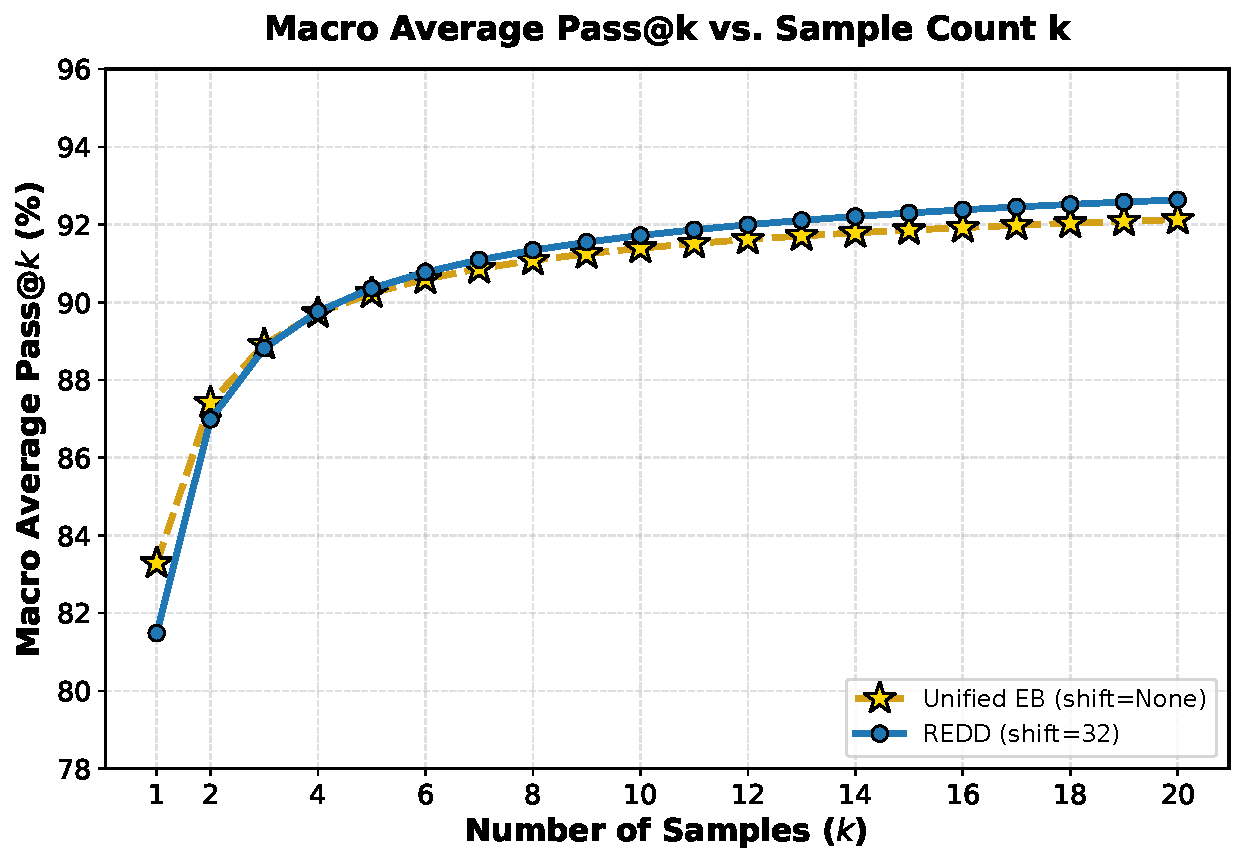
\includegraphics[width=\linewidth]{images/fig_macro_pass_at_k.pdf}
\captionof{figure}{\textbf{Macro Average Pass@$k$ vs.\ Sample Count $k$}. While Unified EB achieves higher Pass@1, RES ($s=32$; ``Rolling'' in the legend) exhibits stronger multi-sample scaling, overtaking Unified EB at $k \ge 6$ to reach $93.58\%$ Pass@20 while running $+31.3\%$ faster.}
\label{fig:macro_pass_at_k}

\end{minipage}
\par\vspace{12pt}
\begin{minipage}{\textwidth}
\centering
    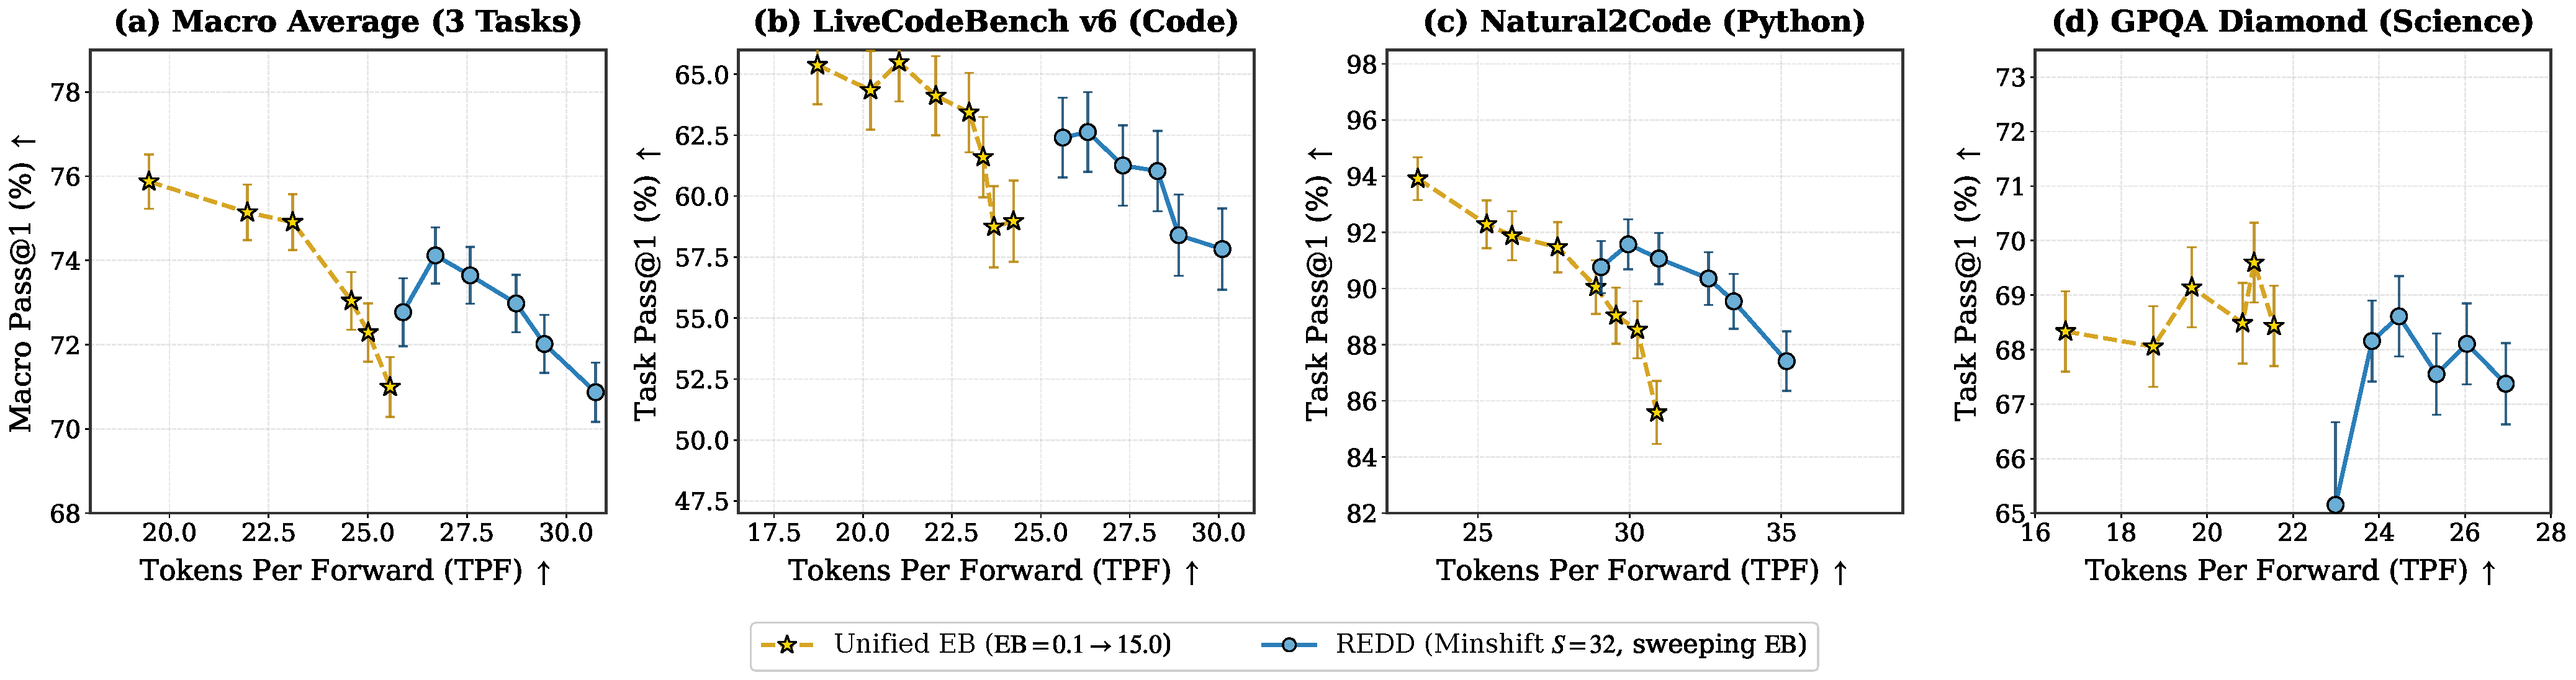
\includegraphics[width=\linewidth]{images/fig_merged_minshift32_eb01_1x4_row.pdf}
    \captionof{figure}{Pareto frontiers of RES with minimum shift $s=32$ (``Merged Sampler'') and Unified EB (``Standard EB Baseline'') under varied EB bounds $.05 \to 1.0$ for LCB v6 and Natural2Code with 5 seed averages, and GPQA Diamond with 20 seed averages due to high noise in the eval.}
    \label{fig:minshift-16}

\end{minipage}
\end{minipage}
\end{lrbox}

\subsection{Main Results}
We compare RES against Unified EB on seven benchmarks at the default entropy bound $\gamma = 0.1$, averaging over 20 seeds (5 for LiveCodeBench).
Table~\ref{tab:eb_unified_vs_rolling} reports accuracy and tokens per forward pass (TPF).
In the figure legends, RES appears as ``Rolling'' or ``Merged Sampler'', and Unified EB as ``EB Unified'' or ``Standard EB Baseline''.

\begin{figure}[tbp]
\centering
\usebox{\resultspanels}
\end{figure}


\paragraph{Performance and Efficiency}
RES raises TPF on every benchmark, by 23\% to 43\%, and \textbf{by 32.5\% on the macro average} (19.3 to 25.5).
Macro accuracy falls by 1.9 points, from 80.7\% to 78.8\%.
The cost is uneven across tasks.
Accuracy rises on MMLU ($+2.5$ points) and is unchanged within confidence intervals on GPQA Diamond; it falls by 0.5 to 2.8 points on GSM8k, HiddenMath, Natural2Code, and LiveCodeBench; and it falls by 10.7 points on IFEval, the one task where RES is clearly worse.
Excluding IFEval, the macro drop is 0.5 points.
One possible cause of the degradation is exposure bias: RES induces a noise pattern across the window that is heavily left-to-right, which is distinct from the homogeneous noise level used within the block at training time.
We do not test this explanation here.

\subsection{Speed-Quality Frontier}
We next sweep both knobs of RES, using the macro-average across LCB v6, GPQA Diamond, and Natural2Code.

\begin{figure}[tbp]
    \centering
    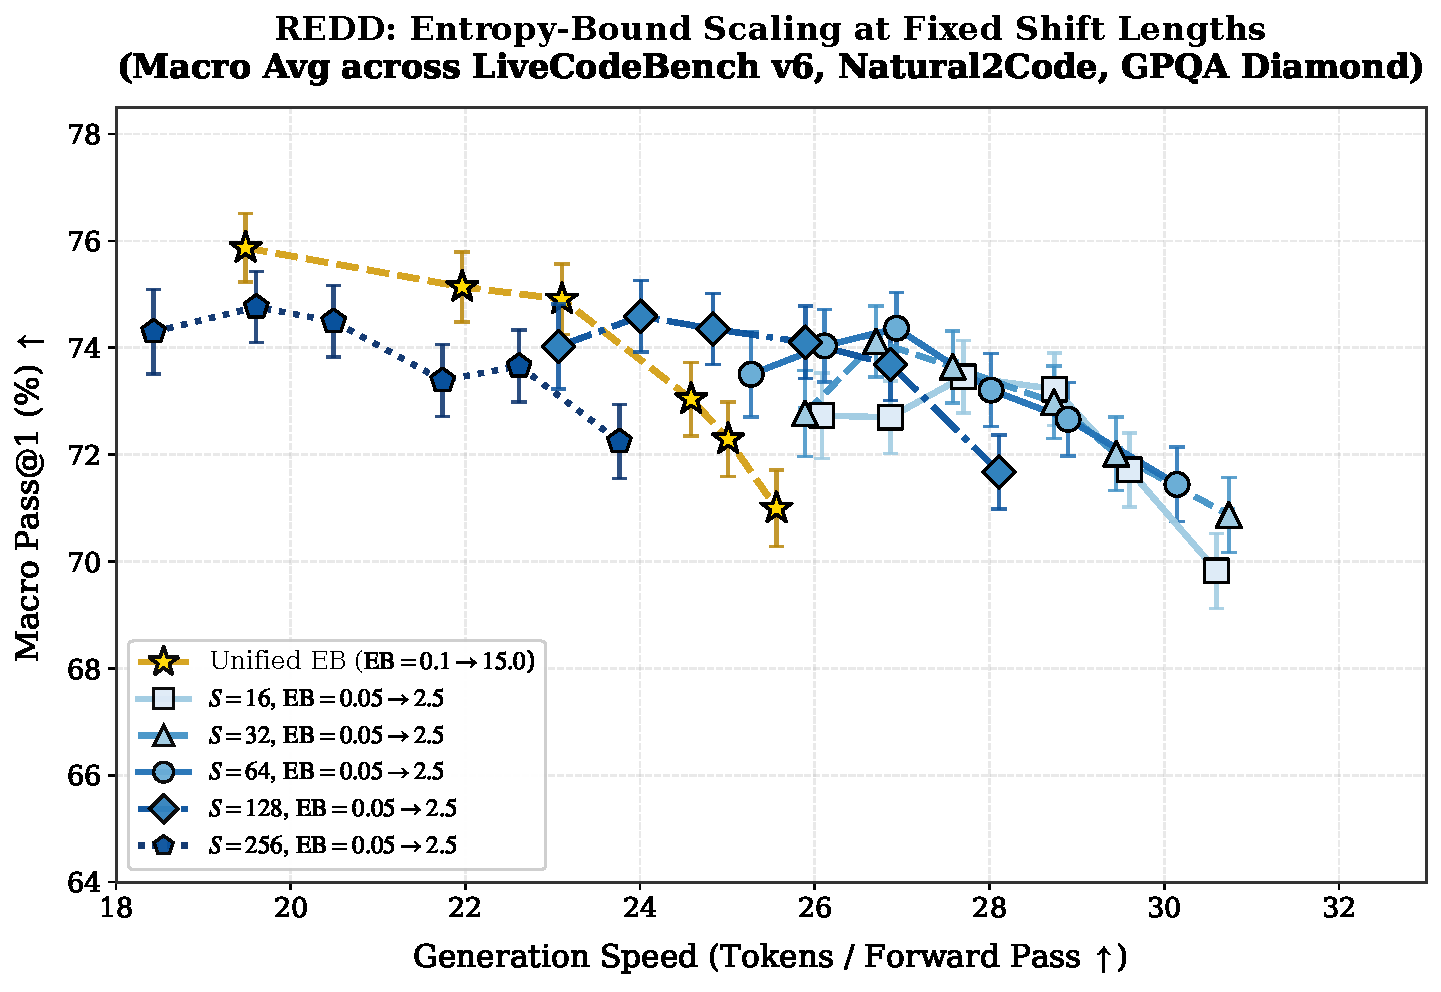
\includegraphics[width=0.6\linewidth]{images/fig_merged_minshift_by_eb_macro.pdf}
    \caption{Frontiers obtained by varying both the minimum shift $s$ in $F_{commit}$ (``S'' in the legend) and the entropy bound in $F_{route}$ for RES (``Merged Sampler''). Small shifts extend the frontier to higher throughput than Unified EB (``Standard EB Baseline'') reaches.}
    \label{fig:dual-frontier}
\end{figure}

\paragraph{Entropy-Bound Sweep}
We sweep the entropy bound for RES with minimum shift $s=32$ and for Unified EB, and show the frontiers in Figure~\ref{fig:minshift-16}.
Relaxing the entropy bound alone takes Unified EB to about 25.5 TPF, where macro Pass@1 has fallen to about 71\%.
At a similar speed RES holds about 74\%, and it reaches the same 71\% only at about 31 TPF.
The gain is in the high-throughput regime: below about 23 TPF Unified EB remains the better choice, so RES extends the frontier rather than dominating it.

\paragraph{Minimum Shift Sweep}
While Unified EB has one axis to trade off performance and speed, RES has the minimum shift in addition to the entropy bound.
Figure~\ref{fig:dual-frontier} shows the frontier for each minimum shift.
Minimum shifts of 16 to 64 give similar frontiers, between about 26 and 31 TPF.
Larger shifts move the frontier toward lower throughput: $s=128$ covers about 23 to 28 TPF, and $s=256$ about 18 to 24 TPF.
This direction is expected, as a larger minimum shift forces the model to spend more time denoising the current span of text in the window.
In this sweep the largest shift does not recover the accuracy of Unified EB at low throughput, so we recommend small shifts for the high-throughput regime and Unified EB otherwise.

\subsection{Multi-Sample Performance}
RES also scales better with the number of samples (Figure~\ref{fig:macro_pass_at_k}).
Unified EB has the higher Pass@1, but RES with $s=32$ overtakes it from $k \ge 6$ samples and reaches 93.58\% Pass@20.
We hypothesize that the EB sampler avoids making ``difficult'' decisions, as it always accepts the lowest entropy positions first.
In contrast, the rolling mechanism along with the position-based temperature schedule enforces a left-to-right generation bias, which was shown in \citet{ni2026flexibility} to improve diversity across generations.


\section{Related Works}
\label{sec:adjacentworks}
Here we discuss works that are closely related to the framework and sampler modifications proposed in this work.

\subsection{Adaptive Block Samplers}
Our work is not the first to suggest incrementally moving the denoising window: \citet{luo2026dsb} applies this to masked diffusion and sees performance gains.
\citet{gat2025set} fine-tunes an auto-regressive model to simultaneously decode the masked tokens ahead using the EB sampler of \citet{ben2026accelerated} while generating the next token auto-regressively, which is the same core idea of a rolling denoising window.
Furthermore, the denoising window is entirely defined by the entropy bound, which has been already defined in \citet{ben2026accelerated} and used in the original sampler of \citet{team2026diffusiongemma}.

Similar ideas of combining diffusion with the left-to-right bias of language have appeared even earlier, such as in \citep{wu2023ar}.
Our contribution is therefore not the rolling window itself, but the separation of acceptance from commitment.
The incremental samplers above freeze a token when it is accepted (Table~\ref{tab:samplers}); under uniform diffusion, RES leaves accepted positions outside the committed prefix free to change.

\subsection{Rolling at Training Time: Clock Diffusion}
Concurrent with our work, \citet{schiff2026clock} introduce Clock Diffusion, which develops essentially the same idea for Gaussian diffusion: a window that rolls left to right and commits finished positions to the KV cache, with a position-dependent noise schedule that mirrors our position-based temperature schedule.
Unlike RES, which is training-free, Clock Diffusion builds this pattern into training and reports strong results, so further aligning the inference process with training represents a very fruitful direction.

\subsection{Rolling Diffusion Beyond Text}
Beyond text generation, the idea of rolling diffusion has been studied extensively in other domains.
Within video generation, rolling diffusion was a natural mechanism to address the temporal nature of video generation and avoid performing diffusion on every frame simultaneously \citep{ruhe2024rolling}. 
Many other works include similar mechanisms \citep{chen2024diffusion, song2025history, xie2025progressive}, and \citet{papa2026asyncpatch} carry the idea over to images by assigning different patches different levels of corruption.


\section{Conclusion}
We separated two choices that diffusion language samplers usually tie together: where each position's next token comes from, and when the position is committed to the KV cache.
On DiffusionGemma, both extremes of the second choice are costly.
Treating acceptance as commitment removes the model's ability to correct itself, which it does without renoising; delaying commitment until the block converges spends over half of the late denoising slots on tokens that are already final.
RES commits the accepted prefix once it is long enough and leaves the rest of the window free to change, which raises tokens per forward pass by 32\% at an average cost of 1.9 points of accuracy and extends the speed-quality frontier at high throughput.
The cost is not uniform: instruction following degrades more than the other tasks, and at low throughput the block sampler remains the better choice.
We hope that the separation of acceptance from commitment serves as a useful baseline for future diffusion samplers.


\section*{Acknowledgments}
We thank Kelly He for thoughtful advice and input; Justin Deschenaux, Valentin De Bortoli, Alexandre Galashov, and Yazid Janati for all hands support; and Abel Gurung for insightful technical discussions.
\FloatBarrier
\begingroup
\small
\setlength{\bibsep}{4pt}
\setlength{\parskip}{0pt}
\bibliography{iclr2025_conference}
\bibliographystyle{iclr2025_conference}
\endgroup

\clearpage
\appendix
\section{Appendix}

\subsection{Computation of Order Statistics}
\label{app:order-stats}
Here we provide details on how the order statistics in Figure~\ref{fig:wasted} (top row) are calculated. 

\paragraph{Acceptance Event}
To track the ordering for the Unified EB sampler, we look at the first
acceptance per position, as the standard entropy bound of $0.1$ results in
positions rarely changing after the first acceptance. Concretely, for a
canvas of $b$ positions $X_1,\dots,X_b$ denoised over $T$ steps, we record
for each position the step at which it is first accepted,
\begin{equation}
  c_i \;=\; \min\bigl\{\, t \in \{1,\dots,T\} \;:\; X_i \text{ is accepted at step } t \,\bigr\},
\end{equation}
setting $c_i = T$ for the rare positions never accepted. Each generated
canvas therefore yields a acceptance-step vector $c \in \{1,\dots,T\}^{b}$. A
purely autoregressive sampler would produce $c_i = i$, so we measure how
closely $c$ tracks the left-to-right index.

\paragraph{Resolving Ties}
Since our goal is to compare the ranking of positions based on acceptance
step, there must be a way to resolve the ties between tokens that are
accepted on the same step. To resolve this, we take the approach of
averaging the order ranking across slots that are tied, assigning each
position the fractional midrank
\begin{equation}
  r_i \;=\; \bigl|\{\,k : c_k < c_i\,\}\bigr|
        \;+\; \tfrac{1}{2}\bigl(1 + \bigl|\{\,k : c_k = c_i\,\}\bigr|\bigr).
\end{equation}
Given the list of acceptance steps $c = [1, 3, 1, 2, 3, 3]$, we first sort them
in ascending order, $[1, 1, 2, 3, 3, 3]$. The positions accepted on the
first step occupy the first and second ranking slots, so both are assigned
the average rank $1.5$; likewise the three positions accepted on the third
step occupy slots four through six and are each assigned $5$. Returning
these ranks to their original positions yields
$r = [1.5,\, 5,\, 1.5,\, 3,\, 5,\, 5]$. Averaging within tie groups keeps
tied positions exchangeable, so the statistic does not depend on an
arbitrary tie-breaking order, and preserves the rank sum
$\sum_i r_i = b(b+1)/2$.

\paragraph{Spearman $\rho$}
Given the vector of rankings, we compare it against the standard
left-to-right rankings $[1, 2, \dots, b-1, b]$ and take the Pearson
correlation coefficient to be the Spearman rank correlation $\rho$. Writing
$\pi_i = i$ for the reference ranking,
\begin{equation}
  \rho \;=\;
  \frac{\sum_{i=1}^{b} (\pi_i - \bar{\pi})(r_i - \bar{r})}
       {\sqrt{\sum_{i=1}^{b} (\pi_i - \bar{\pi})^{2}}\;
        \sqrt{\sum_{i=1}^{b} (r_i - \bar{r})^{2}}},
  \qquad \bar{\pi} = \bar{r} = \frac{b+1}{2}.
\end{equation}
We use this general form rather than the familiar
$1 - 6\sum_i d_i^{2}/\bigl(b(b^{2}-1)\bigr)$, which is valid only when the
ranks are untied.

\paragraph{Kendall $\tau$}
Spearman rank correlation may not reflect the true behavior, as it is
quadratic in terms of the differences per position. Thus we also calculate
the Kendall $\tau$, as it counts inversions and is thus less sensitive to
large differences. More specifically, for every position pair $(X_i, X_j)$
with $i < j$, the pair is \emph{concordant} if $X_i$ was accepted earlier
than $X_j$, \emph{discordant} if $X_j$ was accepted earlier, and
\emph{tied} if both were accepted on the same step. Over all
$n_0 = \binom{b}{2}$ pairs we count
\begin{equation}
  n_c = \bigl|\{(i,j) : i<j,\; c_i < c_j\}\bigr|, \quad
  n_d = \bigl|\{(i,j) : i<j,\; c_i > c_j\}\bigr|, \quad
  n_t = n_0 - n_c - n_d .
\end{equation}
Because the reference ranking is strictly increasing, it contributes no
ties of its own, and every tied pair is tied in acceptance step. We report the
tie-corrected $\tau_b$, which normalises by the pairs whose order is
resolvable at all,
\begin{equation}
  \tau_b \;=\; \frac{n_c - n_d}{\sqrt{n_0\,(n_0 - n_2)}},
  \qquad
  n_2 \;=\; \sum_{s=1}^{T} \binom{m_s}{2},
\end{equation}
where $m_s$ is the number of positions first accepted at step $s$. We
additionally report the pairwise left-to-right agreement rate, which counts
ties as half-agreements,
\begin{equation}
  P_{\mathrm{l2r}} \;=\; \frac{n_c + \tfrac{1}{2} n_t}{n_0},
\end{equation}
equal to $50\%$ under a random acceptance order and $100\%$ under a purely
left-to-right one.

\paragraph{KDE Estimate}
To get the shape of the distribution, we use the default KDE estimator in matplotlib. 

% \begin{figure}
    \centering
    \includegraphics[width=\linewidth]{images/fig6_first_acceptance_position_scatter.pdf}
    \caption{Scatter plot showing the first accept in the trajectory (y axis) against the position within the canvas (x axis) for both tokens that realize their final identity immediately (top row) v.s tokens that fluctuate between the first acceptance and the final canvas (bottom row).}
    \label{fig:acc_vs_pos}
\end{figure}
% \begin{figure}
    \centering
    \includegraphics[width=\linewidth]{images/fig4_first_acceptance_realization.pdf}
    \caption{Histogram of behavior of positions after first acceptance in EB rule. While the majority of the positions stay the same after their first acceptance, a non trivial amount do change from the initially accepted token. This introduces the potential for performance deterioration.}
    \label{fig:placeholder}
\end{figure}
% \begin{figure}
    \centering
    \includegraphics[width=\linewidth]{images/fig5_first_acceptance_timing_histogram.pdf}
    \caption{Histogram of when the first acceptance for tokens tends to occur in the denoising trajectory, organized by tokens that realize their final token identity by the first acceptance (top row) and tokens that change (bottom row). As visible, both tend to overlap very heavily, meaning that there is no clear heuristic to distinguish between whether a position has changed to its final identity or a transient state.}
    \label{fig:acc_vs_timing}
\end{figure}
\end{document}
